% This must be in the first 5 lines to tell arXiv to use pdfLaTeX, which is strongly recommended.
\pdfoutput=1
% In particular, the hyperref package requires pdfLaTeX in order to break URLs across lines.

\documentclass[11pt]{article}

% Change "review" to "final" to generate the final (sometimes called camera-ready) version.
% Change to "preprint" to generate a non-anonymous version with page numbers.
\usepackage[preprint]{acl}

% Standard package includes
\usepackage{times}
\usepackage{latexsym}
\usepackage{amsmath}
\usepackage{listings}
\lstset{
  basicstyle=\ttfamily,
  breaklines=true
}


% For proper rendering and hyphenation of words containing Latin characters (including in bib files)
\usepackage[T1]{fontenc}
% For Vietnamese characters
% \usepackage[T5]{fontenc}
% See https://www.latex-project.org/help/documentation/encguide.pdf for other character sets

% This assumes your files are encoded as UTF8
\usepackage[utf8]{inputenc}
\newcommand{\cmark}{\ding{51}}%
\newcommand{\xmark}{\ding{55}}%
\usepackage{booktabs}
\usepackage{cleveref}
\usepackage{graphicx}
\usepackage{multirow}
\usepackage{tablefootnote}
\usepackage{caption}
\usepackage{subcaption}
\usepackage{url}
\usepackage{makecell}
\usepackage{color,colortbl}
\usepackage{enumitem}
\newcommand\blfootnote[1]{%
  \begingroup
  \renewcommand\thefootnote{}\footnote{#1}%
  \addtocounter{footnote}{-1}%
  \endgroup
}
\usepackage{hyperref}

\newcommand{\csj}[1]{\textcolor{blue}{[Sijie: #1]}}

% This is not strictly necessary, and may be commented out,
% but it will improve the layout of the manuscript,
% and will typically save some space.
\usepackage{microtype}

% This is also not strictly necessary, and may be commented out.
% However, it will improve the aesthetics of text in
% the typewriter font.
\usepackage{inconsolata}

% If the title and author information does not fit in the area allocated, uncomment the following
%
% \setlength\titlebox{6cm}
%
% and set <dim> to something 5cm or larger.

\title{StableToolBench: Towards Stable Large-Scale Benchmarking on \\
Tool Learning of Large Language Models}

% Author information can be set in various styles:
% For several authors from the same institution:
\author{
Zhicheng Guo$\textsuperscript{\rm $1,2$}$,
Sijie Cheng$\textsuperscript{\rm $1,2,3$}$, 
Hao Wang$\textsuperscript{\rm $4$}$, Shihao Liang$\textsuperscript{\rm $5$}$, Yujia Qin$\textsuperscript{\rm $1$}$, \\
\textbf{Peng Li}$\textsuperscript{\rm $2$}$,
\textbf{Zhiyuan Liu}$\textsuperscript{\rm $1$}$,
\textbf{Maosong Sun}$\textsuperscript{\rm $1$}$,
\textbf{Yang Liu}$^{1,2,6}$
\\
 $\textsuperscript{\rm $1$}$Dept. of Comp. Sci. \& Tech., Institute for AI, Tsinghua University, Beijing, China\\
 $\textsuperscript{\rm $2$}$Institute for AI Industry Research (AIR), Tsinghua University, Beijing, China \\
 % $\textsuperscript{\rm $3$}$Beijing National Research Center for Information Science and Technology \\
 $\textsuperscript{\rm $3$}$01.AI  $\textsuperscript{\rm $4$}$Google
 $\textsuperscript{\rm $5$}$The University of Hong Kong \\
  % $\textsuperscript{\rm $6$}$Shanghai Artificial Intelligence Laboratory, Shanghai, China \\
  $\textsuperscript{\rm $6$}$Jiangsu Collaborative Innovation Center for Language Competence, Jiangsu, China \\
 \{\texttt{guo-zc21}, \texttt{csj23}\}\texttt{@mails.tsinghua.edu.cn}
}


% if the names do not fit well on one line use
%         Author 1 \\ {\bf Author 2} \\ ... \\ {\bf Author n} \\
% For authors from different institutions:
% \author{Author 1 \\ Address line \\  ... \\ Address line
%         \And  ... \And
%         Author n \\ Address line \\ ... \\ Address line}
% To start a separate ``row'' of authors use \AND, as in
% \author{Author 1 \\ Address line \\  ... \\ Address line
%         \AND
%         Author 2 \\ Address line \\ ... \\ Address line \And
%         Author 3 \\ Address line \\ ... \\ Address line}

% \author{First Author \\
%   Affiliation / Address line 1 \\
%   Affiliation / Address line 2 \\
%   Affiliation / Address line 3 \\
%   \texttt{email@domain} \\\And
%   Second Author \\
%   Affiliation / Address line 1 \\
%   Affiliation / Address line 2 \\
%   Affiliation / Address line 3 \\
%   \texttt{email@domain} \\}

\begin{document}
\maketitle
\begin{abstract}
% This document is a supplement to the general instructions for *ACL authors. It contains instructions for using the \LaTeX{} style files for ACL conferences. 
% The document itself conforms to its own specifications, and is therefore an example of what your manuscript should look like.
% These instructions should be used both for papers submitted for review and for final versions of accepted papers.
% This document is a supplement to the general instructions for *ACL authors. It contains instructions for using the \LaTeX{} style files for ACL conferences. 
% The document itself conforms to its own specifications, and is therefore an example of what your manuscript should look like.
% These instructions should be used both for papers submitted for review and for final versions of accepted papers.
% This document is a supplement to the general instructions for *ACL authors. It contains instructions for using the \LaTeX{} style files for ACL conferences.
Large Language Models (LLMs) have witnessed remarkable advancements in recent years, prompting the exploration of tool learning, which integrates LLMs with external tools to address diverse real-world challenges. Assessing the capability of LLMs to utilise tools necessitates large-scale and stable benchmarks. However, previous works relied on either hand-crafted online tools with limited scale, or large-scale real online APIs suffering from instability of API status. To address this problem, we introduce StableToolBench, a benchmark evolving from ToolBench, proposing a virtual API server and stable evaluation system. The virtual API server contains a caching system and API simulators which are complementary to alleviate the change in API status. Meanwhile, the stable evaluation system designs solvable pass and win rates using GPT-4 as the automatic evaluator to eliminate the randomness during evaluation. Experimental results demonstrate the stability of StableToolBench, and further discuss the effectiveness of API simulators, the caching system, and the evaluator system. 
\end{abstract}


\section{Introduction}
% Framework:
% \begin{itemize}
%     \item Tool learning empowers LLM.
%     \item However, how to benchmark LLMs on tool usage remains an open issue. There exists a trade-off between questioning reality (To Be Defined/Changed) and the number of APIs but real-life tool using needs both. Previous works fall on one side.
%     \item We propose a new benchmark that strikes a balance between them. including scenario-based question construction, cache-based large-scale API pool and query satisfaction-oriented evaluation. We also propose a new strong baseline....
% \end{itemize}
% \textbf{\textcolor{red}{Framework:}}


% Large Language Models (LLMs, \citealp{brown2020language, geminiteam2023gemini,openai2023gpt4, touvron2023llama}) have demonstrated considerable achievements across a diverse array of tasks, such as commonsense reasoning~\cite{weng2023large, ling2023deductive} and coding~\cite{chen2021evaluating, rozière2023code}. When augmented with auxiliary tools including online search engines and external computational models, LLMs demonstrate enhanced performance in more complex tasks~\cite{nakano2022webgpt, yao2023react, lu2023chameleon}. Therefore, at the time when tool learning becomes more powerful, benchmarking LLMs in the context of tool learning has been increasingly important.

With the rapid developments of Large Language Models (LLMs; \citealp{brown2020language, geminiteam2023gemini,openai2023gpt4, touvron2023llama}), tool learning which leverage LLMs to schedule a variety of external tools has attracted enormous attention~\cite{nakano2022webgpt, yao2023react, lu2023chameleon}.
\blfootnote{Project: 
\href{https://zhichengg.github.io/stb.github.io/}{\texttt{zhichengg.github.io/stb.github.io/}}}\blfootnote{GitHub: \href{https://github.com/THUNLP-MT/StableToolBench}{\texttt{THUNLP-MT/StableToolBench}}} 
Previous studies~\citep{hao2023toolkengpt, hsieh2023tool, schick2023toolformer, tang2023toolalpaca} aim to augment LLMs with tools to enhance performance on conventional natural language processing (NLP) downstream tasks, while recent work~\citep{qin2023webcpm, NEURIPS2022_82ad13ec_webshop, cai2024large} primarily focus on solving real-world scenarios that require the use of tools.
In general, tool learning complements the capabilities of vanilla LLMs and bridges the gap to real-world applications.


To assess the capability of LLMs to use tools, a series of tool learning benchmarks have been introduced. 
Several pioneering studies have heavily relied on human-crafted offline tools~\cite{gpt4tools, xu2023tool} or hand-selected online tools~\cite{li2023api, li2023apibank, chen2023teval}.
While these tools are high-quality, their scale remains relatively small, thereby limiting their ability to accurately reflect real-world scenarios.
To address this limitation, subsequent studies~\citep{tang2023toolalpaca, ye2024tooleyes, qin2023tool} have advocated for leveraging extensive collections of online tools that span across various domains.
Owing to the increased scale, the automatic evaluation of tool learning has moved closer to real-world scenarios.
However, concerns have been raised regarding the stability of these online tools, which has implications for the reproducibility and comparability of benchmark performance over time\footnote{According to its \href{https://www.oed.com/dictionary/benchmark_n?tab=meaning_and_use}{definition}, benchmarks should remain stable, and the model performance assessed on them must be comparable over time.}. 
For instance, the well-recognised ToolBench\footnote{We use  ToolEval2 in ToolBench as the benchmark.}~\cite{qin2023toolllm} has shown performance discrepancies that cannot be reproduced months after its release, as analysed in ~\Cref{sec:pre_analysis_performance}.
This is even more important when faced with a complex environment, where APIs and tools keep changing while the evaluation should maintain its consistency across time.
% For example, ToolBench~\cite{qin2023toolllm}~\footnotemark[1] and ToolEyes~\cite{ye2024tooleyes} exploit real online tools to make up queries covering various domains for evaluation.
% There exists an impossible triangle between benchmark stability, tool reality and the scalability of the the benchmark. Benchmarks equipped with a large number of real tools or APIs tend to be less stable because these tools can change over time. As a result, performance of a model at different time can be different.
% On the other hand, stable offline tools, relied on manual creation, are often limited in narrow scenarios, which makes it even harder to curate real-world questions.
% One can also manually filter out stable real online APIs. However, this tasks a lot of labor work, resulting in small dataset size  and number of tools.
% \footnotetext[1]{For differentiation, we denote ToolBench for ToolBench~\cite{qin2023toolllm} and ToolBench-X for ToolBench~\cite{xu2023tool} below.}

% \begin{figure}
%     \centering
%     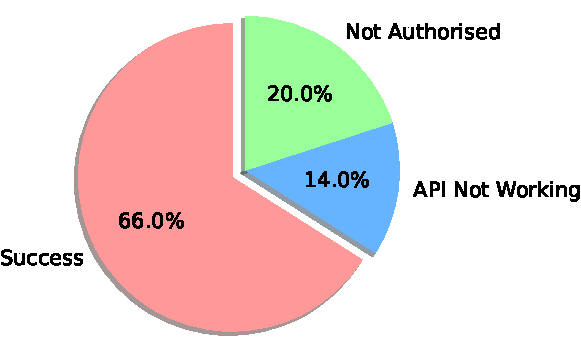
\includegraphics[width=\linewidth]{figs/toolbench_api_statistics.pdf}
%     \caption{API calling statistics in ToolBench. We randomly sample 50 APIs to test the health of these APIs. \textcolor{red}{Add ToolEyes.}}
%     \label{fig:api_statistics}
% \end{figure}

% \begin{minipage}{\textwidth}
% \begin{table*}
%     \centering
%     \resizebox{\linewidth}{!}{
%     \begin{tabular}{lrrcccc}
%         \toprule
%         {\textbf{Benchmarks}} & {\textbf{\#Tools}} & {\textbf{\#APIs}} & {\textbf{Tool Accessibility}}  & {\textbf{\#Queries}}  & \textbf{Metrics}\\
%         % & \textbf{Query Construction} \\
%         \midrule

%         {ToolBench$^x$}~\cite{xu2023tool}&  \phantom{0000,}8 & \phantom{000,}232 & Offline & \phantom{0}2,746  & SR \\
%         {GPT4Tools}~\citep{gpt4tools} & \phantom{000,}22 & \phantom{00000}- & Offline & 41,000 & SR\\
%          {APIBench}~\citep{patil2023gorilla}  & \phantom{0000,}3 & \phantom{00}1,645 & Online & 17,002 & Acc \\
         
%         {T-Eval}~\citep{chen2023teval}  &   \phantom{000,}15 & \phantom{00000}- & Online & \phantom{00,}533 & WR\\
%          {API-Bank}~\citep{li2023apibank} & \phantom{000,}53 & \phantom{00}2,138 & Online & \phantom{00,}274 & Acc/RL\\
%          {ToolAlpaca}~\cite{tang2023toolalpaca} &  \phantom{00,}426 & \phantom{00000}- & Online & \phantom{0}3,938 & SR \\

       
%         {ToolEyes}~\cite{ye2024tooleyes}  & \phantom{00,}568 & \phantom{00000}- & Online &  \phantom{00,}382 & Stage-wise Score \\
%         {ToolBench}~\citep{qin2023toolllm}  & 3,451 & 16,464 & Online & 12,657 & PR/WR\\
%         {StableToolBench (Ours)}  & 3,451 & 16,464 &  Online+Offline & 12,657& SoPR/SoWR\\
%         \bottomrule
%     \end{tabular}}
%     \caption{Comparisons between our benchmark and recent benchmarks. SR, Acc, RL, PR, WR, SoPR, and SoWR stands for Success Rate, API Call Accuracy, Pass Rate, Win Rate~\cite{qin2023toolllm} and our proposed Solvable Pass Rate and Solvable Win Rate.}
%     \label{tab:intro_previous_worls}
% \end{table*}
% \end{minipage}


% However, according to its definition\footnote{
% \url{https://www.oed.com/dictionary/benchmark_n?tab=meaning_and_use}}, benchmarks should remain stable, and the model performance assessed on them must be comparable over time. Consequently, there are concerns regarding the reproducibility and comparability of model performance over time when using these large-scale tool learning benchmarks.


Existing large-scale benchmarks may struggle to provide stable evaluations for various reasons. We propose several hypotheses for this issue.
Firstly, the complexity of tasks involving tool usage makes it challenging for the common automatic evaluator, \texttt{gpt-3.5}, to function effectively as a discriminator. As discussed in~\Cref{sta_eval}, the evaluator cannot reliably determine whether a task is solvable or unsolvable, leading to variability in model performance due to this capability limitation.
Secondly, the stability of API status for a significant portion of online tools (55.6\% in ToolBench) is inconsistent. Users may be required to authorise the use of these tools or APIs, and tools provided by developers may be accessible during the initial construction of the benchmark but become unavailable later. This fluctuation further undermines the reliability and reproducibility of model performance assessments over time.
This situation results in a problem where the constructed queries in the benchmarks may no longer be completed with their originally referenced tools. Consequently, it is crucial to strike a balance between enhancing the stability of these benchmarks and maintaining their diversity and scope.

% Firstly, due to the difficulty of complex tasks with tool usage, the common automatic evaluator \texttt{gpt-3.5} can not assume the role of discriminating.
% The automatic evaluator cannot determine whether the task is solvable or unsolvable as discussed in~\Cref{sta_eval}, thus the capability limitation introduces randomness to model performances.
% Secondly, the stability of API status in more than half of online tools (55.6\% in ToolBench) is fluctuant.
% On the one hand, users may be requested to authorise the use of these tools or APIs. 
% On the other hand, these online tools provided by developers may be available during the initial construction of the benchmark but become inaccessible later. 
% some online tools provided by developers may not be available at some point.
% Secondly, usable tools or APIs are subject to updates that can alter their functionality, such as changing required arguments or producing different responses at subsequent times. 
% This leads to a problem where the constructed queries in the benchmarks may no longer be completed with their original referenced tools.
% Therefore, it is crucial to strike a balance between enhancing the stability of these benchmarks and maintaining their diversity and scope.
% As shown in \Cref{fig:api_statistics}, a significant number of APIs are not callable in ToolBench and ToolEyes, due to authorisation or other issues.


% although using real APIs well reflects real life, baseline results may not be reproducible and comparable across time, limiting the use of the benchmarks. 
% Compounding the problem, such queries are hard to discover, even for human, making query filtering infeasible. 


% To this end, we propose a new benchmark, named StableToolBench, which is composed of a virtual API system and a stable evaluation system. 
% In the virtual API system, we first build a caching system to store the output of API calls. This ensures the stability and reproducibility of API behaviours. Given that the benchmark questions are limited, our caching system can cover a significant number of API call scenarios. 
% However, merely using a cache is not enough because there still exists a large number of unavailable APIs. 
% To resolve this problem, we use LLMs to simulate the behaviours of these APIs.
To address these issues, we propose a new benchmark named StableToolBench, which incorporates a virtual API system and a stable evaluation system. 
 We first build a virtual API system to replace the real one. As a start, we build a caching system to store the outputs of API calls. This approach ensures the stability and reproducibility of API behaviours. Given the limited number of benchmark questions, our caching system can cover a significant number of API call scenarios.
% Also, when the API behaviours of real APIs get changed, leading to calling failure, LLMs simulated APIs can serve as stable alternatives.
However, relying solely on a cache is insufficient because many APIs remain unavailable. To resolve this problem, we use large language models (LLMs) to simulate the behaviours of these APIs.
Specifically, we feed the documentation and few-shot real API calls if available in the cache to LLMs and ask LLMs to mock the behaviour of the APIs given a request. 
As a result, users can always get responses from APIs in an indistinguishable way as long as the LLMs are accessible. 
% Note that to mitigate the gap between the behaviours of real and simulated APIs, we use real API calls as the few-shot examples.
% With LLM simulation, behaviours of APIs can change when LLMs change their behaviour, especially when using a closed-source LLM such as GPT-4~\cite{openai2023gpt4}. We store calls to the API system 
% \color{black}
% Nevertheless, differences may exist between the behaviours of real and simulated APIs. To mitigate the gap, we create the simulator by feeding LLMs with API documentation and real API calls so that LLMs can mock real API behaviours well. 
% Experiments show that the simulated APIs can perform in an indistinguishable way from the real ones. 
% It is still crucial to highlight that, considering the irreplaceable nature of the reality provided by real APIs, our system prioritises real API calls.
% .\textcolor{red}{[Experiments follow]}
% Despite stability provided by LLMs, repeatedly calling LLMs can be very expensive. Responses generated by LLMs can also exhibit considerable variability. 
% Therefore, we additionally created an API response cache to store the results of real and simulated APIs. 
On the whole, our system first tries to find a hit in the cache.
Unless there is a cache miss and a real API call is not received, the simulated server will be used.
% The API call will not be directed to real and simulated APIs unless there is a cache miss.
% It is still crucial to highlight that, considering the irreplaceable nature of the reality provided by real APIs, our system prioritises real API calls. Only when a real API call is not received, the simulated server will be used.
% \textbf{(2) The stable evaluation system}. 

We then improve the evaluation system to make it more stable. We design two metrics (i.e., SoPR and SoWR) after judging solvable tasks and replace all the automatic evaluators with \texttt{GPT-4} to mitigate the randomness and indistinguishability during evaluation.
Experiments demonstrate that our virtual API system, when combined with the improved evaluation system, can provide stable evaluation against API modifications. Furthermore, our system exhibits significant reliability in terms of realism, diversity, and documentation following accuracy.
% Experiments demonstrate that our virtual API system consistently maintains stability in the face of real API modifications. Furthermore, our evaluation system yields more stable results and exhibits a high level of concordance with human assessments.
% Experiments show that our virtual API system can provide consistent stability across real API changes. In addition, our evaluation systems provides more stable results and achieves high agreement with human.
% [More Description] This makes it possible to curate real and diverse queries across different scenarios based on a large scale of APIs. [More Description] We also propose to a query-answer based NLI evaluation to better fit the real-world queries.

\begin{figure}[t!]
    \centering
    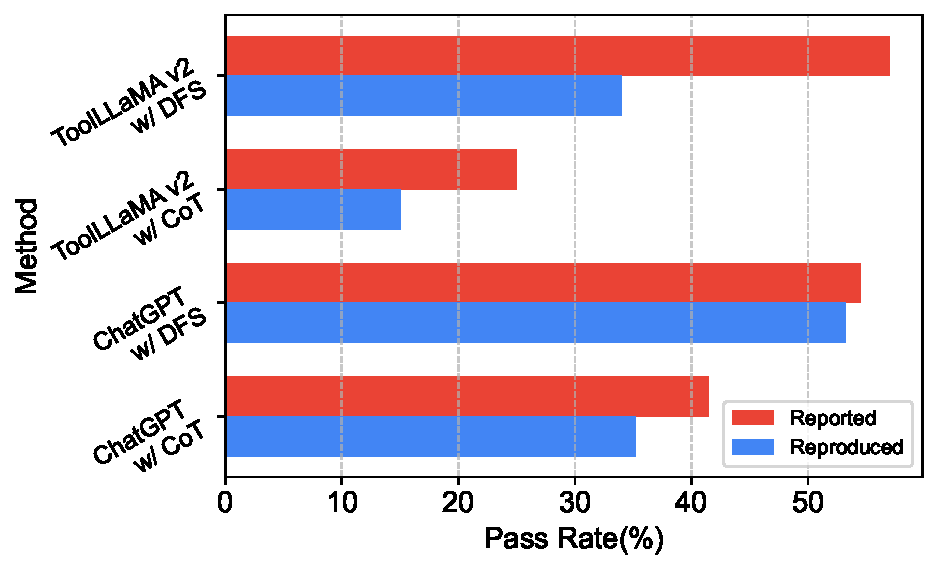
\includegraphics[width=\linewidth]{figs/real_comparison.pdf}
    \caption{Comparison of performance (Pass Rate) reported in the paper and reproduced by us on the I1-Instruction group of ToolBench.}
    \label{fig:performance_comparison_failure}
\end{figure}
The main contributions of our work are summarised as follows:
\begin{itemize}[noitemsep]
    \item A tool-learning benchmark featured a large number of cached stable simulated APIs, well-balancing stability and reality of the APIs and much more stable evaluation metrics.
    \item Extensive experiments show that our benchmark provides much more stable model performance, robust to various types of API failures.
    \item Besides enhanced stability, our virtual API system exhibits reality, diversity and reliability comparable to that of the real API system.
\end{itemize}




\section{Stability Analysis on ToolBench}
In this section, we initiate a comprehensive analysis to reveal the stability of established tool benchmarks, using Toolbench~\citep{qin2023tool} as a case study.
We examine the stability of ToolBench by investigating three key dimensions: performance, evaluation, and API status.

\subsection{Stability of Performance}\label{sec:pre_analysis_performance}

Benchmarks are designed to consistently evaluate the performance of various models over time.
To test this consistency, we reproduce the model performances and record any variations.
Our study employs Chain-of-Thought (CoT;~\citealp{wei2023chainofthought}) and Depth First Search (DFS) strategies, leveraging ChatGPT and ToolLLaMA for comparative analysis.
We adhere strictly to the configurations detailed in ToolBench, utilising the ChatGPT version \texttt{gpt-3.5-turbo-0613} and \texttt{ToolLLaMA-v2}.
As depicted in \Cref{fig:performance_comparison_failure}, we compare the original Pass Rates for the I1-Instruction group reported by ToolBench with the Pass Rates we reproduced for four conventional methods.
\begin{figure}[]
    \centering
    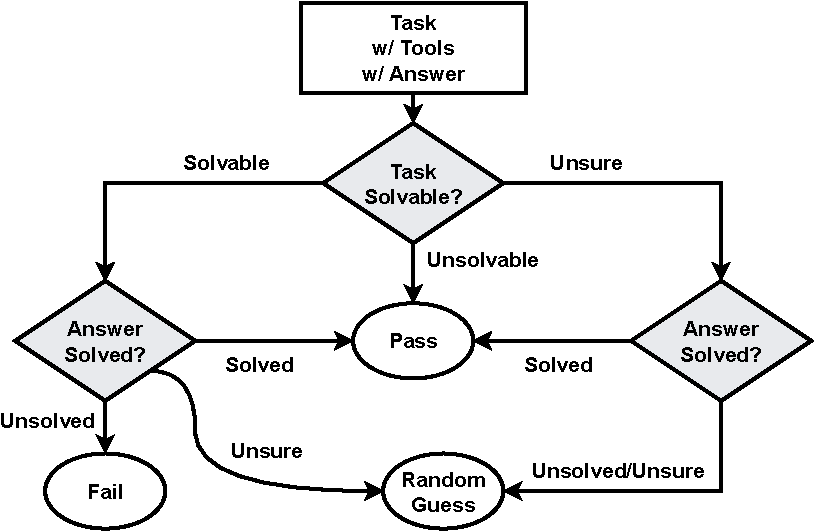
\includegraphics[width=\linewidth]{figs/PR.pdf}
    \caption{Pass Rate evaluation in ToolBench paper.}
    \label{fig:pass-rate}
\end{figure}
Our findings indicate a notable decline in the performance of all methods over time, which raises concerns about the stability of ToolBench as a benchmark.



% \begin{figure*}
%     % \centering
%     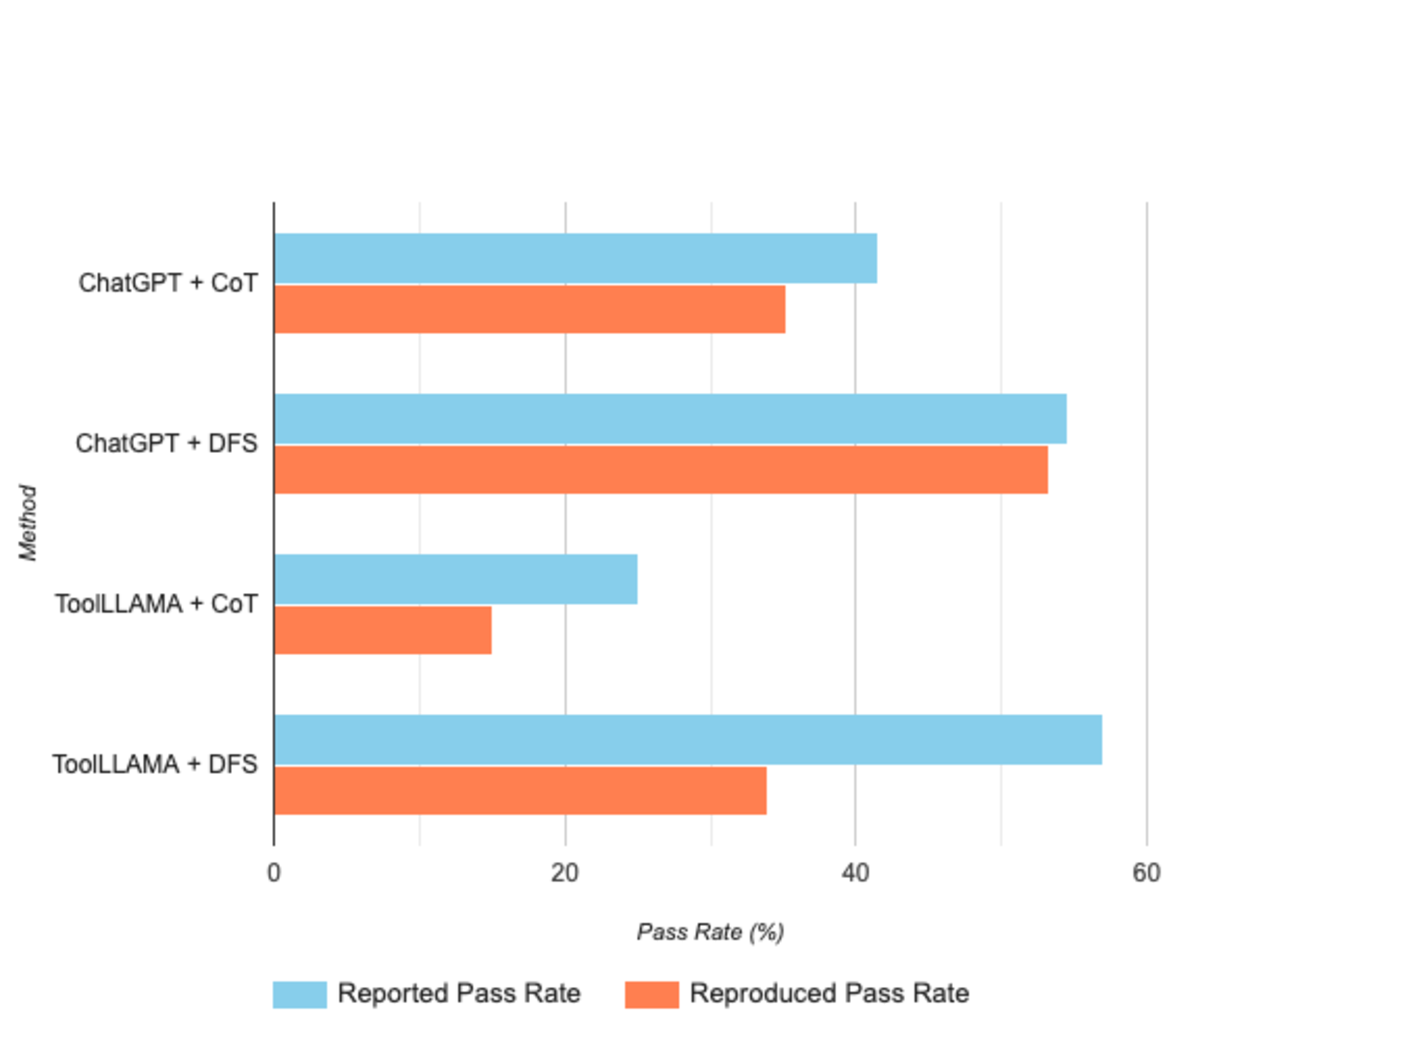
\includegraphics[width=\textwidth]{figs/table_2_perf_comparison.pdf} 
%     \caption{Comparison of performance (Pass Rate) reported in the paper and reproduced by us of ChatGPT and ToolLLaMA v2 on the I1-Instruction group of ToolBench.}
%     \label{tab:performance_comparison}
% \end{figure*}


\subsection{Stability of Evaluation}
\label{sta_eval}

In ToolBench, there are two types of metrics, including Pass Rate (PR) and Win Rate (WR). 
% PR is automatically evaluated by \texttt{gpt-3.5-turbo-16k}.
PR is calculated based on using \texttt{gpt-3.5-turbo-16k} to determine if a task is solvable and whether the generated answer can solve the corresponding task.
% PR is then calculated based on the solvability of the task and the effectiveness of the answer.
% The statuses of tasks are categorized as solvable, unsolvable, or unsure, while the statuses of answers can be solved, unsolved, or unsure.
\Cref{fig:pass-rate} details the computation process of PR.
Specifically, a solvable task results in a pass if the answer is solved, a failure if unsolved, and is randomly determined if unsure.
For tasks deemed unsure, a pass is assigned only if the answer is solved; otherwise, a random outcome is chosen.
If a task is unsolvable, the result defaults to a pass regardless of the answer status.
Moreover, WR is derived from the comparative PR of paired candidates.
% as shown in~\Cref{todo}.
A candidate's WR increases by one each time it passes while the other fails.
In all other situations, WR relies on \texttt{gpt-3.5-turbo-16k} to automatically evaluate the paired candidates.

% Please add the following required packages to your document preamble:
% \usepackage{multirow}
% Please add the following required packages to your document preamble:
% \usepackage{multirow}
% \begin{table}[]
% \small
% \centering
% \begin{tabular}{l|l|l|c|l}
% \toprule
%  & \multicolumn{3}{c}{\textbf{Task Status}} \\
%  & Solvable & \multicolumn{1}{l}{Unsolvable} & Unsure \\
%  \cmidrule
% Solved & Passed & \multirow{3}{*}{Passed} & Passed \\
% Unsolved & Failed &  & \multirow{2}{*}{Random} \\
% Unsure & Random &  &\\
% \bottomrule
% \end{tabular}
% \end{table}



\begin{table}[t!]
    \small
    \centering
    \resizebox{\linewidth}{!}{
    \begin{tabular}{l|ccc|ccc|c|c}
    \toprule
    \multirow{2}{*}{\textbf{Method}} & \multicolumn{3}{c|}{\textbf{Task}} & \multicolumn{3}{c|}{\textbf{Answer}} & \multirow{2}{*}{\textbf{Pass}} & \multirow{2}{*}{\textbf{Win}} \\
    & S & US & UE & S & US & UE & & \\
    \midrule
        \multirow{3}{*}{CoT} & 168 & 23 & 9 & 19 & 170 & 11 & 33.0 & 50.0 \\
         & 165 & 29 & 6 & 16 & 174 & 10 & 31.5 & 46.5 \\
         & 151 & 40 & 9 & 20 & 167 & 13 & 37.5 & 53.0 \\
        \midrule
        \multirow{3}{*}{DFS} & 116 & 68 & 16 & 17 & 167 & 16 & 50.5 & 54.0 \\
         & 122 & 59 & 19 & 20 & 162 & 18 & 46.5 & 48.0 \\
         & 132 & 54 & 14 & 22 & 157 & 21 & 55.0 & 56.0 \\
    \bottomrule
    \end{tabular}}
    \caption{Experiments use \texttt{GPT-3.5-Turbo-0613} with CoT and DFS. S, US, and UE indicate solvable (solved), unsolvable (unsolved), and unsure. Pass and Win denote pass rate and win rate, respectively. Win rates are evaluated against the first run of CoT. This experiment is run on 4 Feb 2024.}
    \label{tab:sta_eval}
\end{table}

To assess the stability of evaluation, we perform both CoT and DFS using \texttt{gpt-3.5-turbo-0613} on the I1-Instruction group dataset. 
These analyses are conducted using the provided tools and repeat over three iterations each.
The resulting PR and WR are presented in~\Cref{tab:sta_eval}, with detailed task and answer items.
% Although DFS generally exhibits higher PR than CoT, the distribution of tasks and answers is illogical.
Despite PRs of DFS being generally higher than CoT, the contribution of the task is larger than the answer.
However, it is worth noting that the tasks are the same in both CoT and DFS, where their results are expected to be consistent.
On the contrary, the discrimination of answers between CoT and DFS is weak, where a considerable proportion are unsolved.
Moreover, WR does not reflect the same trend as PR, where the second run of WR in DFS (48.0) is even lower than the first run of CoT.
Therefore, all the phenomena reflect that \texttt{gpt-3.5-turbo-16k} can not assume the role of the automatic evaluator in tool learning, which will be discussed in~\Cref{sec:evaluator}.


% \begin{figure}[h!]
%     \centering  
%      \begin{subfigure}[b]{\linewidth}
%         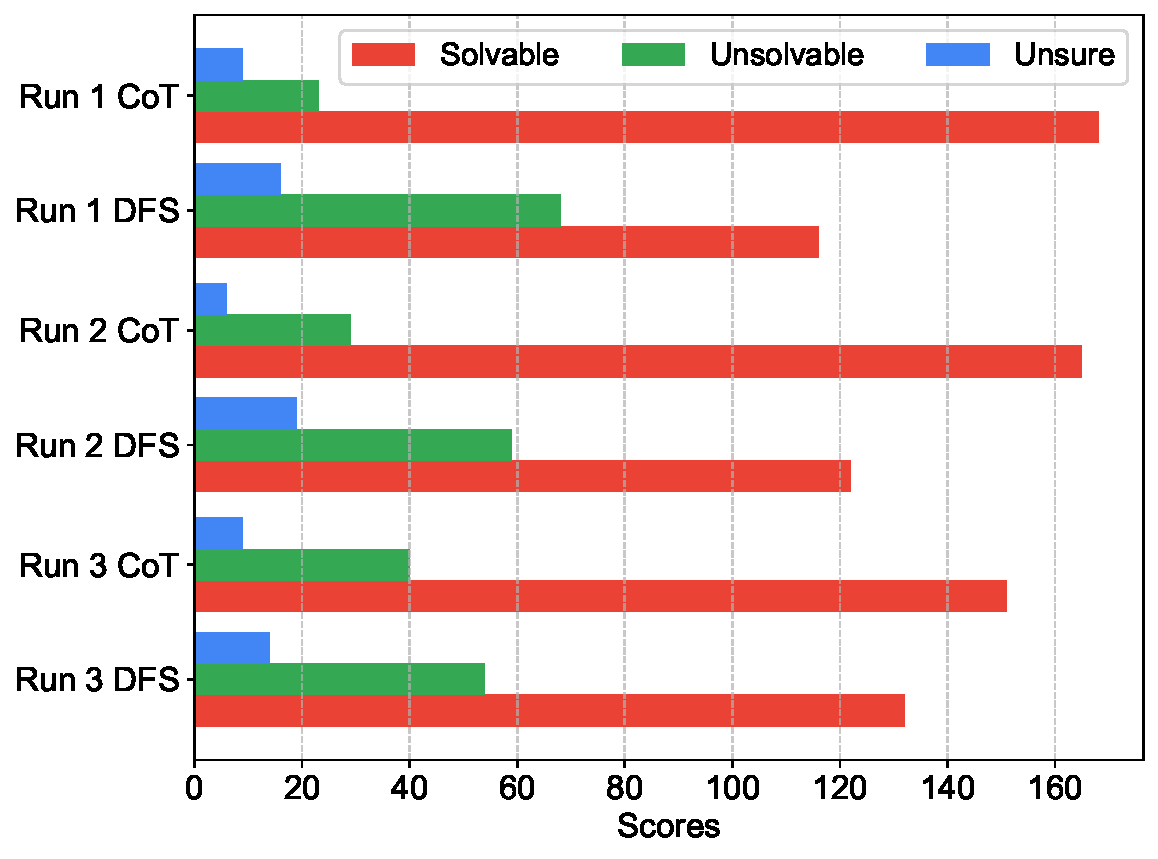
\includegraphics[width=\linewidth]{figs/task_status_count.pdf}
%         \caption{Task Status}
%       \end{subfigure}
%       \begin{subfigure}[b]{\linewidth}
%     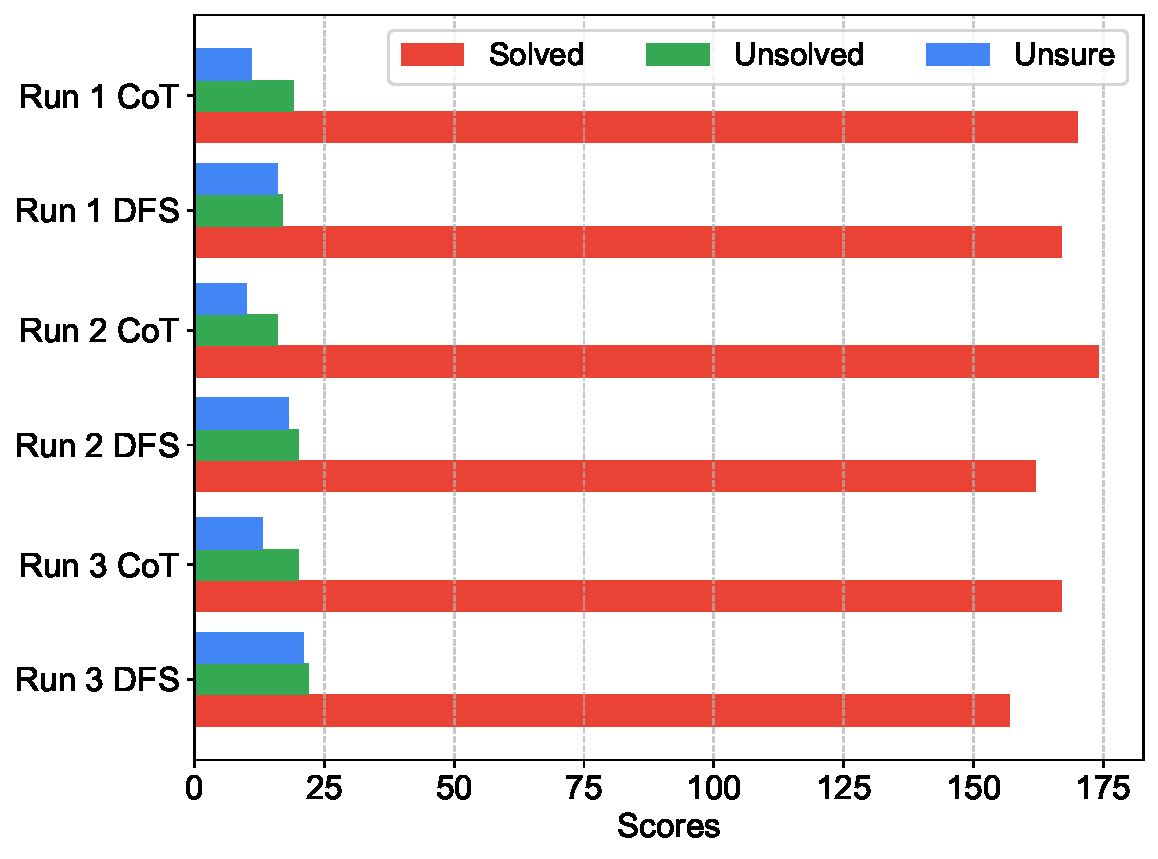
\includegraphics[width=\linewidth]{figs/answer_status_count.pdf}
%     \caption{Answer Status}
%       \end{subfigure}
    
%     \caption{Task and Answer status}
%     \label{fig:sta_eval}
% \end{figure}

% \begin{figure}[ht!]
%     \centering
%     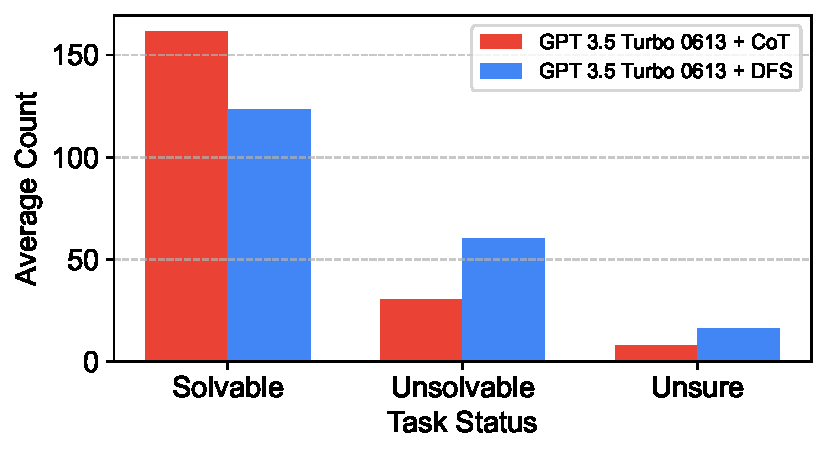
\includegraphics[width=\linewidth]{figs/status_eval.pdf}
%     \caption{Task and Answer status}
%     \label{fig:sta_eval}
% \end{figure}




\subsection{Stability of API Status}
\label{api_status}
% \textcolor{red}{Discuss the phenomenon that APIs are not callable in ToolBench and ToolEyes. These are resulting from authentication, documentation change, etc}.
% Results shown in \Cref{fig:toolbench-api-status}.
% To find the causes of the aforementioned instability,
We investigate the change of API status in ToolBench. 
In detail, we scan the original APIs downloaded from ToolBench, and use \texttt{gpt-4-turbo} to automatically write calls via the prompts as shown in \Cref{app:prompt_make_call}.
According to the keyword in API feedback, we classify these APIs into three categories: success, not availability, and not authorisation\footnote{Note that we use the \texttt{toolbench-key} provided in ToolBench to simulate the real running process in the benchmark.}.
The API status and the detailed errors of not availability are presented in \Cref{fig:api_change_info}. 
\begin{figure}[]
    \centering   
    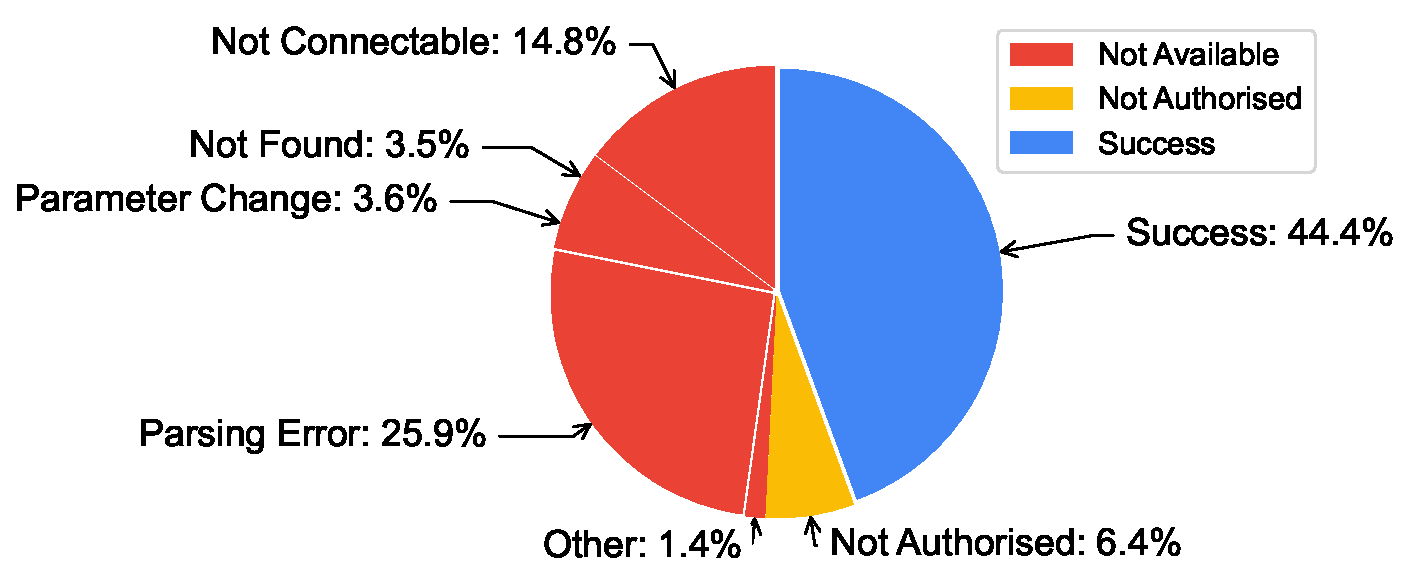
\includegraphics[width=\linewidth]{figs/api_status_merged.pdf}
    \caption{Statistics of API changes. Parsing errors are caused by post-processing errors of local API documentation, which have been solved in our benchmark.}
   
    \label{fig:api_change_info}
\end{figure}
As can be seen, only 44.4\% of API calls are successful, while other API calls are mostly not available with various errors and some are not authorised.

% As for the not available APIs, xxx.

% authentication: 1058
% request_failure: 2426
% parameter: 591
% not_working: 248
% not_found: 583
% bugs: 4247




% \begin{table}[h!]
%     \centering
%     \small
%     \begin{tabular}{cc}
%      \toprule
%     \textbf{Status Type} & \textbf{Percentage} (\%) \\
%     \midrule
%     % No Change & 83.3 \\
%     % Parameter Change & 16.7 \\
%         No Change & 84.5 \\
%     Parameter Change & 15.5 \\
%      \bottomrule
%     \end{tabular}
%     \caption{APIs changed in ToolBench.}
%     \label{tab:api_change}
% \end{table}
\begin{figure}[h!]
    \centering
    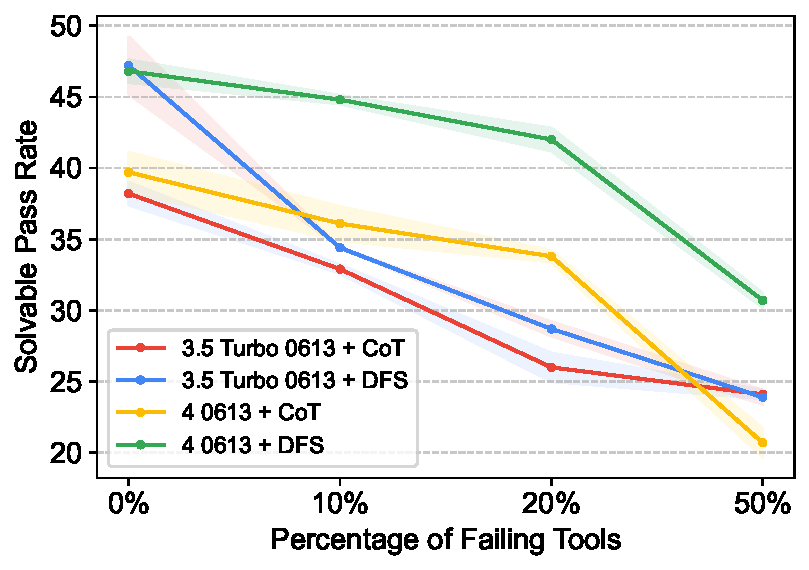
\includegraphics[width=\linewidth]{figs/real_solving_scores.pdf}
    \caption{Solvable Pass Rate (SoPR) change when manually making APIs down on the I1 Instruction group.}
    \label{fig:real_api_stability_test}
\end{figure}


\begin{figure*}[t!]
    \centering
    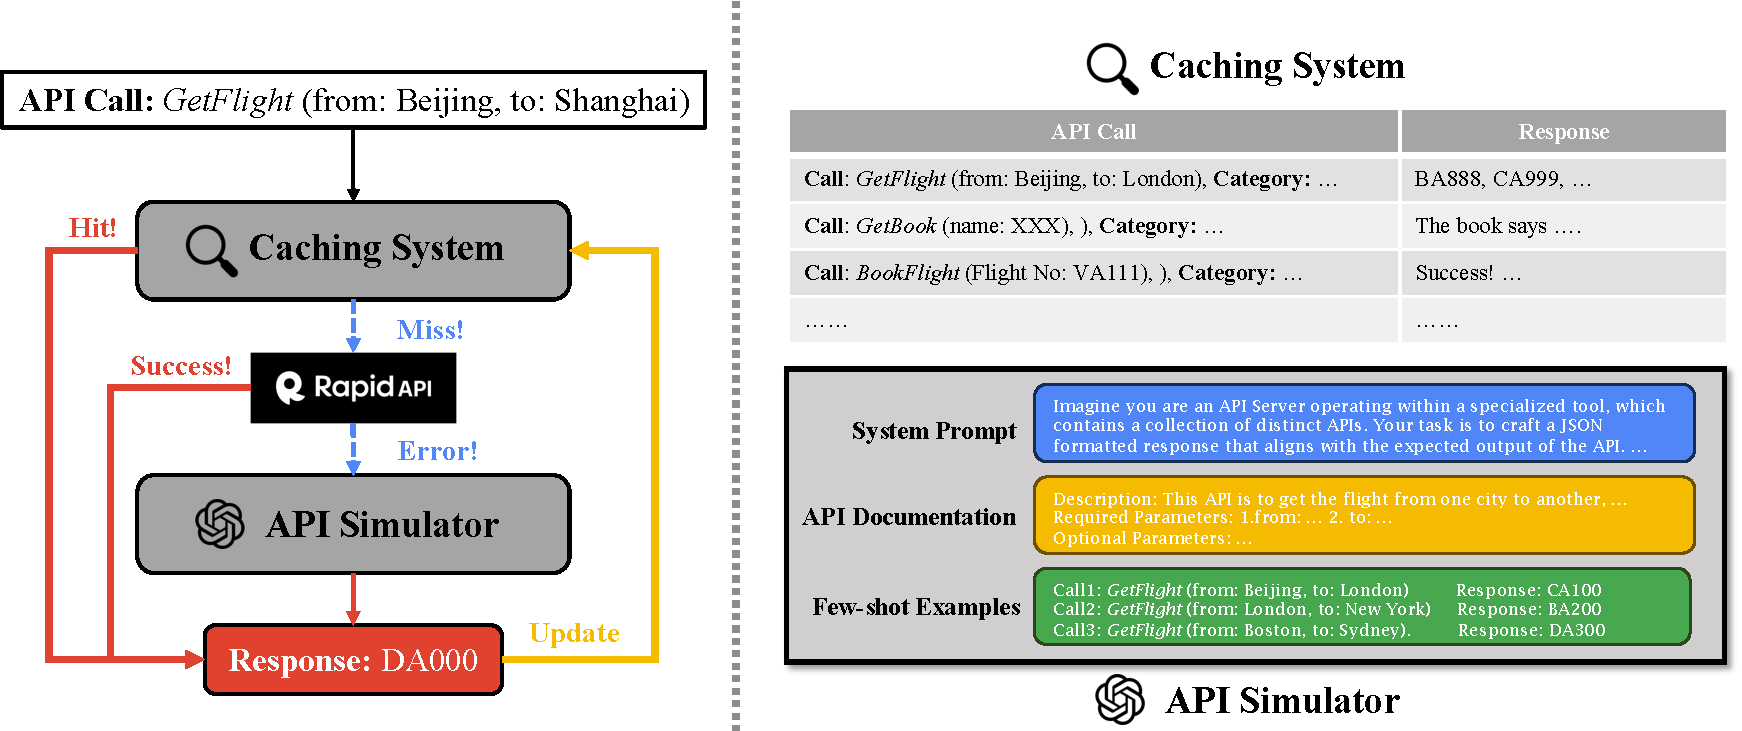
\includegraphics[width=\textwidth]{figs/main_figure.pdf} 
    \caption{The process of calling APIs in our proposed virtual API server.}
    \label{fig:main_figure}
\end{figure*}


% \begin{figure}[h!]
%     \centering
%     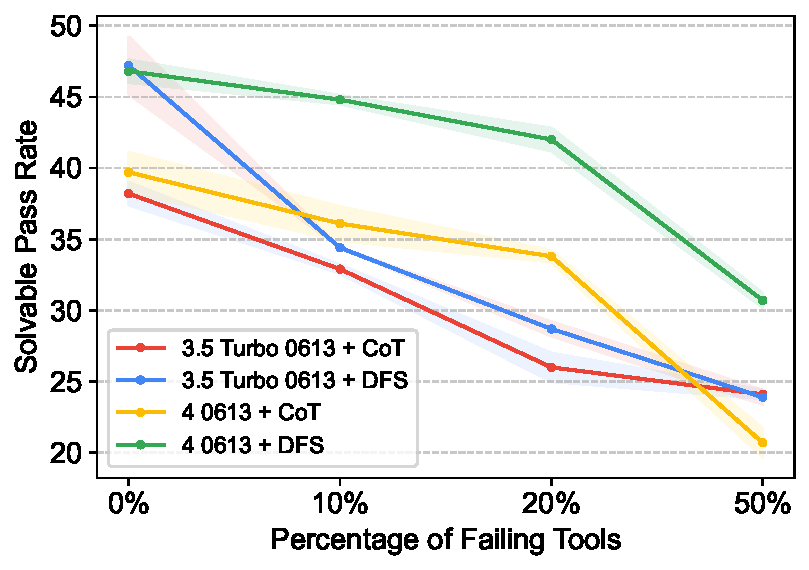
\includegraphics[width=\linewidth]{figs/real_solving_scores.pdf}
%     \caption{Solvable Pass Rate (SoPR) change when manually making APIs down on the I1 Instruction group.}
%     \label{fig:real_api_stability_test}
% \end{figure}
Furthermore, to validate the impact of API call failures on the stability of model performance, we manually make some success tools\footnote{In ToolBench, a tool is composed of several APIs. For example, a database tool can have two APIs: a writing API and a reading API. } down by returning a special failure call. Specifically, we randomly sample a proportion of success tools containing success APIs found in \Cref{fig:api_change_info}.
At testing time, when sampled tools are called, a special response will be thrown: \texttt{\{``error'': ``'', ``response'': ``This API did not return any useful information...''\}} to simulate the API call failures. 
We conduct baseline models with different proportions (i.e., 0\%, 10\%, 20\%, and 50\%) of sampled APIs on the I1 Instruction set.
% To confirm that the sampled tools will be called, we calculate the proportions of ground truth tools appearing in the sampled tools. 
% The results are shown in \Cref{app:proportion_sampling}.
Due to the issues in evaluation, we use our stable evaluation system proposed in~\Cref{sec:evaluation_system} as the same as our main experiments.
For each experiment, we evaluate three times and report the average scores as shown in \Cref{fig:real_api_stability_test}.
It can be seen that the performance degrades a lot when the proportion of successful APIs is down, thus the impact of API status on stability is considerable.

% \begin{figure}[h!]
%     \centering
%     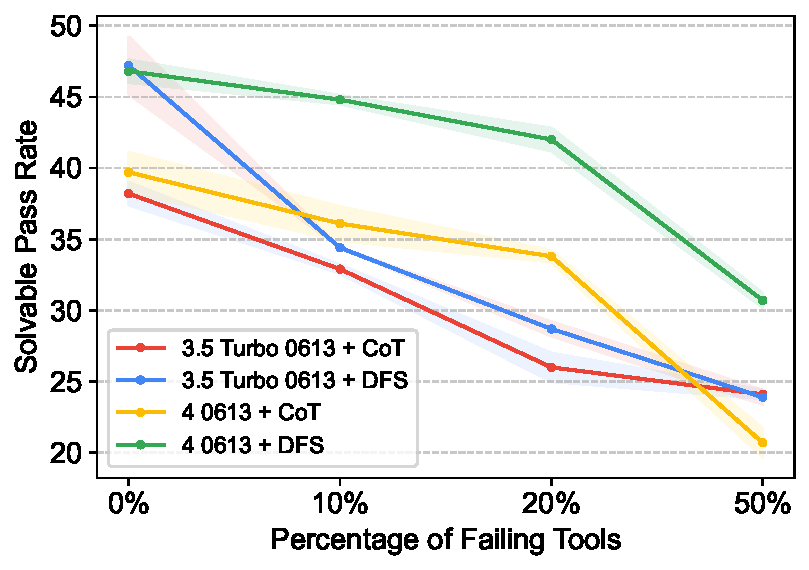
\includegraphics[width=\linewidth]{figs/real_solving_scores.pdf}
%     \caption{Solvable Pass Rate (SoPR) change when manually making APIs down on the I1 Instruction group.}
%     \label{fig:real_api_stability_test}
% \end{figure}

% \subsection{Stability of API Document}

% It is worth noting that we can only simulate functions calling varying very small parts of parameters, thus there may be other parameter errors.
% Therefore, secondly, we directly investigate into the parameter changes in all API documentation over time.
% % sample 50 APIs used in ToolBench and 
% We crawl the current document corresponding to the API in Toolbench from RapidAPI\footnote{\url{https://rapidapi.com}}. 
% Then, we check whether the parameter information of these APIs is changed and the results on parameter changes are shown in \Cref{tab:api_change}. It shows that a significant portion (16.7\%) of APIs change their documentation, which may affect the stability of model performance.

% \begin{figure}
%     \centering
%     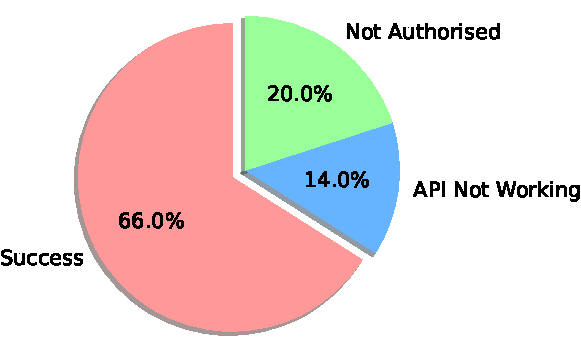
\includegraphics[width=\linewidth]{figs/toolbench_api_statistics.pdf}
%     \caption{API status in ToolBench. We sample 50 APIs in the APIs used in ToolBench and manually label the status of these APIs.}
%     \label{fig:toolbench-api-status}
% \end{figure}

% We manually let some APIs down to test the impact of API stability on model performance. [Experimental Setups] Results are shown in \Cref{tab:real_api_stability_test}.[Results analysis] 



% \begin{table}[]
%     \centering
%     \small
%     \begin{tabular}{cccc}
%         \toprule
%         \multirow{2}{*}{\textbf{Method}} & \multicolumn{3}{c}{\textbf{Percentage of Failing APIs}}\\
%         % \cmidrule{2-5}
%           & 10\% & 20\% & 50\% \\
%         \midrule
%          ChatGPT + CoT & 47.5 & 49.5 & 32.5 \\
%          ChatGPT + DFS & 47.0 & 46.0 & 34.5  \\
%          ToolLLaMA + CoT & 48.0 & 47.0 \\
%          ToolLLaMA + DFS & 50.5 & 50.5 \\
%          \bottomrule
%     \end{tabular}
%     \caption{Win rate against no change when manually make APIs down on the I1 Instruction group.}
%     \label{tab:real_api_stability_test}
% \end{table}


\section{StableToolBench}


Considering that stability is a crucial feature of benchmarking, in this paper, we specifically design a virtual API server and stable evaluation system to improve the stability based on ToolBench, and propose a new benchmark, named StableToolBench.

\subsection{Virtual API Server}

With real APIs, many of the failures encountered when reproducing its experiments are caused by expired APIs, network issues, or failed authentication.
To address this problem, we specifically propose a virtual API server with two components as illustrated in~\Cref{fig:main_figure}, including a caching system and API simulator.
Moreover, we design API calling rules to combine these two components to ensure the virtual API server is stable.



\paragraph{Caching System.}

We first implement a caching system that stores responses of all API callings to ensure consistency.
The caching system uses keys composed of their category, tool, API name, and arguments.
As a start, we populate the initial cache using the API call history from the training data and the reproduced test data released in ToolBench\footnote{\url{https://drive.google.com/drive/folders/1yBUQ732mPu-KclJnuQELEhtKakdXFc3J}}.
% We also update the cache with the reproduced test data released in ToolBench.
% New responses will be continuously recorded when running the experiment.
To ensure the quality of cached APIs, only valid records following the rule in \Cref{app:filter_rule} will be saved.
It is worth noting that we will also reserve some APIs with exceptions to keep the reality.
In this way, most API responses will be readily available, allowing the benchmark focus on probing the tool usage ability of designed methods with minimal impact on tool availability.
Furthermore, the API call in new experiments will also be continuously updated in the cache to ensure scalability.
The statistics of cache are shown in \Cref{tab:cache_components}.
\begin{table}[h!]
    \centering
    \small
    \begin{tabular}{lcccc}
        \toprule
         \textbf{Source} & \textbf{Train Set} & \textbf{Test Set} & \textbf{New Exp} & \textbf{Total} \\
         \midrule
         \textbf{Before} & 58,105 & 5,921 & 255,828 & 352,630 \\
         \textbf{After} & 25,995 & 2,393 & 136,592 & 164,980 \\
         \bottomrule
    \end{tabular}
    \caption{Cache components and their sizes before and after filtration. The cache of new experiments is updated until 12 Feb 2024.}
    \label{tab:cache_components}
\end{table}
Additionally, as an extra benefit, this approach reduces the latency introduced by interacting with real APIs, and also saves the costs for the API simulator discussed below.
% The caching system ultimately accumulates a total of 164,980 items, comprising 25,995 items sourced from training data, 5,921 items derived from testing data, with the remainder originating from our collection and various experimental runs.

%  \begin{table*}[t!]
%     \centering
%     \small
%     \resizebox{\textwidth}{!}{
%     \begin{tabular}{lccccccc}
%         \toprule
%         \textbf{Method} & \textbf{I1 Instruction} & \textbf{I1 Category} & \textbf{I1 Tool} & \textbf{I2 Category} & \textbf{I2 Instruction} & \textbf{I3 Instruction} & \textbf{Average} \\
%         \midrule

%     3.5 0613 (C) & 55.9{\tiny $\pm{1.0}$} & 50.8{\tiny $\pm{0.8}$} & 55.9{\tiny $\pm{1.0}$} & 44.1{\tiny $\pm{0.8}$} & 36.2{\tiny $\pm{0.4}$} & 51.4{\tiny $\pm{1.5}$} & 49.1{\tiny $\pm{1.0}$} \\
%     3.5 0613 (D) & 66.4{\tiny $\pm{1.5}$} & 64.3{\tiny $\pm{1.0}$} & 67.2{\tiny $\pm{2.4}$} & 67.7{\tiny $\pm{0.8}$} & 61.5{\tiny $\pm{1.0}$} & 81.4{\tiny $\pm{1.5}$} & 68.1{\tiny $\pm{1.4}$} \\
%     4 0613 (C) & 50.7{\tiny $\pm{0.4}$} & 57.1{\tiny $\pm{0.3}$} & 51.9{\tiny $\pm{0.3}$} & 55.0{\tiny $\pm{1.1}$} & 61.6{\tiny $\pm{0.8}$} & 56.3{\tiny $\pm{0.8}$} & 55.4{\tiny $\pm{0.6}$} \\
%     4 0613 (D) & 65.5{\tiny $\pm{1.1}$} & 62.0{\tiny $\pm{1.7}$} & 72.1{\tiny $\pm{1.6}$} & \textbf{70.8}{\tiny $\pm{1.3}$} & \textbf{73.1}{\tiny $\pm{1.4}$} & 74.9{\tiny $\pm{1.5}$} & 69.7{\tiny $\pm{1.4}$} \\
%     T-LLaMA (C) & 37.2{\tiny $\pm{0.1}$} & 42.3{\tiny $\pm{0.4}$} & 43.0{\tiny $\pm{0.5}$} & 37.4{\tiny $\pm{0.4}$} & 33.6{\tiny $\pm{1.2}$} & 39.6{\tiny $\pm{1.0}$} & 38.9{\tiny $\pm{0.6}$} \\
%     T-LLaMA (D) & 59.8{\tiny $\pm{1.5}$} & 59.5{\tiny $\pm{1.4}$} & 65.7{\tiny $\pm{1.1}$} & 56.5{\tiny $\pm{0.3}$} & 47.6{\tiny $\pm{0.4}$} & 62.8{\tiny $\pm{1.9}$} & 58.7{\tiny $\pm{1.1}$} \\
%     \midrule
%     3.5 1106 (C) & 51.3{\tiny $\pm{0.6}$} & 48.8{\tiny $\pm{0.3}$} & 59.9{\tiny $\pm{0.8}$} & 50.8{\tiny $\pm{0.7}$} & 43.2{\tiny $\pm{0.8}$} & 58.5{\tiny $\pm{0.8}$} & 52.1{\tiny $\pm{0.7}$} \\
%     3.5 1106 (D) & 67.8{\tiny $\pm{0.9}$} & 67.2{\tiny $\pm{0.3}$} & \textbf{72.9}{\tiny $\pm{0.7}$} & 63.2{\tiny $\pm{1.0}$} & 70.9{\tiny $\pm{0.4}$} & 77.6{\tiny $\pm{0.8}$} & 69.9{\tiny $\pm{0.7}$} \\
%     4 Turbo (C) & 63.1{\tiny $\pm{1.0}$} & 64.5{\tiny $\pm{0.5}$} & 55.3{\tiny $\pm{0.3}$} & 63.0{\tiny $\pm{0.8}$} & 57.3{\tiny $\pm{0.8}$} & 61.7{\tiny $\pm{0.8}$} & 60.8{\tiny $\pm{0.7}$} \\
%     4 Turbo (D) & \textbf{70.8}{\tiny $\pm{1.0}$} & \textbf{71.1}{\tiny $\pm{0.7}$} & 70.4{\tiny $\pm{1.2}$} & 70.4{\tiny $\pm{1.3}$} & 71.7{\tiny $\pm{0.4}$} & \textbf{84.7}{\tiny $\pm{1.7}$} & \textbf{73.2}{\tiny $\pm{1.1}$} \\

%          \bottomrule
%     \end{tabular}
%     }
%     \caption{Solvable pass rate scores. We run all models once, evaluate three times and take the average results. ``3.5 0613'', ``4 0613'', ``3.5 1106'', ``4 Trubo'', ``T-LLaMA'' stands for \texttt{gpt-3.5-turbo-0613}, \texttt{gpt-4-0613}, \texttt{gpt-3.5-turbo-1106}, \texttt{gpt-4-turbo-preview}, 
%     \texttt{ToolLLaMA v2} respectively. C and D stand for CoT and DFS respectively. The experiments below follow the denotation.}
%     \label{tab:main_sopr}
% \end{table*}


\paragraph{API Simulator.}
Due to the limited coverage of the caching system, we propose to use LLMs to simulate API responses that are not in the cache and unavailable. 
Specifically, we ask \texttt{gpt-4-turbo} to simulate the API behaviour based on the original documentation in ToolBench.
The API documentation includes the descriptions of the functions and their corresponding parameters. 
% incorporate the documentation in the prompt of GPT-4 to generate a response given a requested input.
To mitigate the difference between simulated and real APIs, we use real API calls in the caching system as few-shot examples~\citep{brown2020language} for the LLM to better mock the behaviours. 
% These examples are sampled from previous calls on the same API stored in the caching system.
We keep the maximum number of examples at five.
When less than five examples exist in the cache, all of them will be used.
Detailed prompts can be found in \Cref{app:prompt_simulation}.
\begin{figure}[t!]
    \centering
    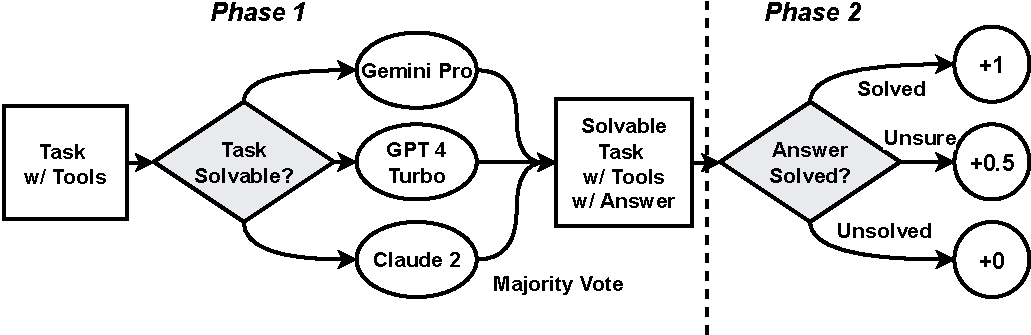
\includegraphics[width=\linewidth]{figs/SoPR.pdf}
    \caption{The process of our SoPR evaluation.}
    \label{fig:SoPR}
\end{figure}


\paragraph{API Calling Rules.}
Based on the caching system and the API simulator, we create API calling rules to ensure the stability of the virtual API server.
When a call request $(\mathrm{e},\mathrm{args})$, where $\mathrm{e}$ is the API endpoint and $\mathrm{args}$ is the arguments for that endpoint, is received, the system will first search the caching system for $(\mathrm{e},\mathrm{args})$ pair.
If a cache hit exists, the cached response will be directly returned.
When there is a cache miss, then the system will try to call the real API for a response to maintain the reality of the whole system.
If the real API calling is successful, the response will be returned.
However, when the caching system does not contain and the real API is not available, the system will finally call the simulated API. 
The final response whether from the real API or the simulated API will be saved to update in the caching system.
% Note that this will not affect the performance because all models evaluated will use the same response to a call whenever the the first call is made.

\subsection{Stable Evaluation System}
\label{sec:evaluation_system}

In this section, we propose a two-phase evaluation process, including judging solvable tasks and evaluating with two metrics, as shown in~\Cref{fig:SoPR}. Moreover, we replace all the automatic evaluators with \texttt{gpt-4-turbo}.

\paragraph{Judging Solvable Tasks.}\label{sec:judge_solvable_tasks}
\begin{table}[t!]
  \centering
  \small
  \resizebox{\linewidth}{!}{
  \begin{tabular}{lccccccc}
    \toprule
    & \textbf{I1-I} & \textbf{I1-C} & \textbf{I1-T} & \textbf{I2-I} & \textbf{I2-C} & \textbf{I3-I} & \textbf{Total}\\
    \midrule
    \textbf{Full} & 200 & 200 & 200 & 200 & 200 & 100 & 1,100 \\
    \textbf{Solvable} & 163 & 153 & 158 & 106 & 124 & 61 & 765\\
    % \midrule
    % \textbf{Total} & \multicolumn{2}{c}{765} & \multicolumn{3}{c}{1100} \\
    \bottomrule
  \end{tabular}}
  \caption{Statistics of original full and solvable tasks before and after judging. \texttt{C,I,T} stands for the Category, Instruction and Tool subgroup of the test set. Experiments below follow the denotation.}
  \label{tab:task_filteration}
\end{table}
Considering that both unsolvable and unsure tasks would introduce enormous randomness while the results of tasks fluctuate wildly, we try to obtain a fixed collection of solvable tasks to eliminate the problems.
To achieve this, we use three state-of-the-art LLMs, i.e., \texttt{gpt-4-turbo}, \texttt{gemini-pro}, and \texttt{claude-2}, to determine whether a task is solvable or unsolvable.
The prompt is shown in \Cref{app:prompt_task_solvability}.
The task will be judged as solvable when more than two models evaluate it as solvable.
The statistics of solvable tasks across all test datasets in ToolBench are shown in \Cref{tab:task_filteration}. 
% All reported scores are on the solvable tasks in the following experiment section.

\begin{table*}[t!]
    \centering
    \small
    \resizebox{\textwidth}{!}{
    \begin{tabular}{lccccccc}
        \toprule
        \textbf{Method} & \textbf{I1 Instruction} & \textbf{I1 Category} & \textbf{I1 Tool} & \textbf{I2 Category} & \textbf{I2 Instruction} & \textbf{I3 Instruction} & \textbf{Average} \\
        \midrule
     3.5 0613 (C)  & 52.2{\tiny $\pm{1.1}$} & 47.3{\tiny $\pm{0.6}$} & 53.6{\tiny $\pm{1.3}$} & 42.5{\tiny $\pm{2.1}$} & 35.8{\tiny $\pm{2.0}$} & 48.1{\tiny $\pm{0.8}$} & 46.6{\tiny $\pm{1.3}$} \\
    3.5 0613 (C)  & 60.3{\tiny $\pm{1.3}$} & 66.2{\tiny $\pm{1.2}$} & 67.1{\tiny $\pm{0.0}$} & 59.1{\tiny $\pm{0.4}$} & 51.3{\tiny $\pm{1.2}$} & 73.8{\tiny $\pm{2.3}$} & 63.0{\tiny $\pm{1.1}$} \\
    
    4 0613 (C) & 45.5{\tiny $\pm{0.4}$} & 57.4{\tiny $\pm{0.3}$} & 48.8{\tiny $\pm{0.7}$} & 43.0{\tiny $\pm{0.7}$} & 46.5{\tiny $\pm{0.9}$} & 48.1{\tiny $\pm{1.5}$} & 48.2{\tiny $\pm{0.8}$} \\
    4 0613 (D) & 57.3{\tiny $\pm{0.6}$} & 57.3{\tiny $\pm{0.3}$} & 60.9{\tiny $\pm{1.0}$} & 57.9{\tiny $\pm{1.0}$} & 51.3{\tiny $\pm{0.8}$} & 66.4{\tiny $\pm{2.4}$} & 58.5{\tiny $\pm{1.0}$} \\
    T-LLaMA (C) & 32.3{\tiny $\pm{1.0}$} & 40.3{\tiny $\pm{0.8}$} & 36.7{\tiny $\pm{0.5}$} & 34.7{\tiny $\pm{0.7}$} & 25.2{\tiny $\pm{0.4}$} & 33.9{\tiny $\pm{1.5}$} & 33.9{\tiny $\pm{0.8}$} \\
    T-LLaMA (D) & 44.5{\tiny $\pm{0.9}$} & 49.6{\tiny $\pm{1.3}$} & 48.9{\tiny $\pm{2.7}$} & 50.8{\tiny $\pm{1.1}$} & 31.9{\tiny $\pm{1.9}$} & 53.6{\tiny $\pm{2.0}$} & 46.6{\tiny $\pm{1.7}$} \\
    \midrule
   3.5 1106 (C)& 50.4{\tiny $\pm{0.5}$} & 45.1{\tiny $\pm{1.4}$} & 50.8{\tiny $\pm{0.3}$} & 48.7{\tiny $\pm{0.8}$} & 42.1{\tiny $\pm{0.4}$} & 55.7{\tiny $\pm{0.0}$} & 48.8{\tiny $\pm{0.6}$} \\
    3.5 1106 (D) & 62.8{\tiny $\pm{0.3}$} & 63.9{\tiny $\pm{1.2}$} & 65.6{\tiny $\pm{0.3}$} & 56.5{\tiny $\pm{0.7}$} & 56.9{\tiny $\pm{1.2}$} & 67.2{\tiny $\pm{1.3}$} & 62.2{\tiny $\pm{0.8}$} \\
    4 Turbo (C) & 52.8{\tiny $\pm{1.3}$} & 56.6{\tiny $\pm{0.9}$} & 51.9{\tiny $\pm{0.5}$} & 51.9{\tiny $\pm{1.0}$} & 52.8{\tiny $\pm{0.8}$} & 52.5{\tiny $\pm{0.0}$} & 53.1{\tiny $\pm{0.8}$} \\
    4 Turbo (D) & 59.2{\tiny $\pm{0.5}$} & 61.7{\tiny $\pm{0.7}$} & 65.7{\tiny $\pm{1.0}$} & 55.6{\tiny $\pm{0.6}$} & 55.2{\tiny $\pm{0.4}$} & 66.1{\tiny $\pm{4.3}$} & 60.6{\tiny $\pm{1.3}$} \\

         \bottomrule
    \end{tabular}
    }
    \caption{Solvable pass rate scores. We run all models once, evaluate three times and take the average results. ``3.5 0613'', ``4 0613'', ``3.5 1106'', ``4 Turbo'', ``T-LLaMA'' stands for \texttt{gpt-3.5-turbo-0613}, \texttt{gpt-4-0613}, \texttt{gpt-3.5-turbo-1106}, \texttt{gpt-4-turbo-preview}, 
    \texttt{ToolLLaMA v2} respectively. C and D stand for CoT and DFS respectively. The experiments below follow the denotation. We use \texttt{gpt-4-turbo-2024-04-09} as the evaluator. Evaluation done on May 2024.}
    \label{tab:main_sopr}
\end{table*}




    
% \begin{table}[h!]
%     \centering
%     \small
%     \begin{tabular}{lcc}
%         \toprule
%         \multirow{2}{*}{\textbf{Group}} & \textbf{After} & \textbf{Before} \\
%         & \textbf{Filtration} & \textbf{Filtration}\\
%         \midrule
%         {I1 Instruction} & 163 & 200\\
%         {I1 Category }& 153 & 200 \\
%         {I1 Tool} & 158 & 200 \\
%         {I2 Instruction} & 106 & 200\\
%         {I2 Category} & 124 & 200 \\
%         {I3 Instruction} & 61 & 100 \\
%         \midrule
%         {{Total}} & 765& 1100\\
%         \bottomrule
%     \end{tabular}
%     \caption{Query count statistics before and after filtration. \csj{todo}}
%     \label{tab:task_filteration}
% \end{table}

\paragraph{Metrics.}
We then report Solvable Pass Rate (SoPR) and Solvable Win Rate (SoWR) based on our obtained solvable tasks.
Due to the limitation of \texttt{gpt-3.5-turbo-16k} in tool learning, we uniformly adopt \texttt{gpt-4-turbo} as the automatic evaluator.
SoPR is in essence PR with all tasks solvable and only assesses the answers using the same prompt in ToolBench.
The evaluator assigns outcomes of answers categorised as Solved, Unsolved, or Unsure, which respectively contribute scores of 1, 0.5, and 0 to the overall SoPR calculation.
As for SoWR, when one is solved and the other is unsolved, the solved one wins.
Under other circumstances, \texttt{gpt-4-turbo} will be used to make a win-lose decision.  
% Note that the evaluation will be made whenever an \texttt{Unsure} label occurs.
% When calculating SoPR, the task description, available tools are fed into the automatic evaluator, using the same prompt as that in evaluating answer status when calculating Pass Rate\footnote{Prompts used to evaluate Pass Rate and Win Rate from ToolBench are at \url{https://github.com/OpenBMB/ToolBench/blob/master/toolbench/tooleval/evaluators/tooleval_gpt-3.5-turbo_default/template.txt}}.
% Furthermore, we improved the Win Rate with our SoPR to make it more stable, named Solvable Win Rate (SoWR). 
% Originally, when two methods received a \texttt{Passed} label and a \texttt{Failed} label during Pass Rate evaluations, the one with \texttt{Passed} label always wins when making Win Rate evaluations. Under other circumstances, an LLM based automatic evaluator will be used to make a win-lose decision. 




% \begin{table}[]
%     \centering
%     \small
%     \begin{tabular}{c|cc}
%         \toprule
%         \textbf{Methods} &  \\
%         \midrule
%          GPT 4 Turbo & 74.0 & 78.0\\
%          GPT 3.5 Turbo & 68.0 & 56.0 \\
%          \bottomrule
%     \end{tabular}
%     \caption{Human evaluation on answer solving (for pass rate) and comparison (for win rate).}
%     \label{tab:human_eval_task}
% \end{table}



\section{Experiment}

\subsection{Performance}\label{sec:performance}

% \textcolor{red}{Run different baseline models on the benchmark. The goal is to show that ranking of models on the benchmarks is the same as the precedents, i.e. improved stability will not change discrimination of the benchmark.}
Following ToolBench, we run \texttt{gpt-3.5-0613}, \texttt{gpt-4-0613}, \texttt{ToolLLaMA-v2} with CoT and DFS, replenishing with latest models \texttt{gpt-3.5-1106} and \texttt{gpt-4-turbo}.  
The results of SoPR and SoWR are shown in \Cref{tab:main_sopr,tab:main_sowr}. Generally, GPT-4 series models outperform GPT-3.5 models, while ToolLLaMA performs worst with the same inference algorithm.
Also, DFS significantly outperforms CoT whichever LLMs are used.
These phenomena are consistent with ToolBench.
Furthermore, probably thanks to the improved function calling capabilities, newer GPT models performed better. 
% Nevertheless, with more stable tools, gaps between LLMs are smaller with DFS than with CoT. This may indicate that more trials can significantly boost problem-solving performance.
\begin{table}[t!]
    \centering
    \small
    \resizebox{\linewidth}{!}{
    \begin{tabular}{lccccccc}
        \toprule
        \textbf{Method} & \textbf{I1-I} & \textbf{I1-C} & \textbf{I1-T} & \textbf{I2-I} & \textbf{I2-C} & \textbf{I3-I} & \textbf{Avg} \\
        \midrule
        3.5 0613 (D) & 60.7 & 67.3 & 59.5 & 63.2 & 62.1 & 75.4 & 64.7 \\
        4 0613 (C) & 54.6 & 58.8 & 58.2 &  75.5 & 60.5 & 62.3 & 61.7 \\
        4 0613 (D) & 62.6 & 62.7 & 58.2 & 74.5 &62.9 &  67.2 & 64.7 \\
        T-LLaMA (C) & 31.3 &28.1 &  33.5 & 35.8 & 33.9 &  24.6 & 31.2 \\
        T-LLaMA (D) & 44.8 & 45.8 & 44.3 & 59.4 & 41.1 & 50.8 & 47.7 \\
        \midrule
        3.5 1106 (C) &  47.2 & 47.7 & 44.9 & 50.9 & 54.0 & 62.3 & 51.2 \\
        3.5 1106 (D) & 55.8 &53.6 &  51.9 & 68.9 & 59.7 & 68.9 & 59.8 \\
        4 Turbo (C) & 71.2 &{77.1} &  61.4 & { 79.2} & {71.8} & {67.2} & {71.3} \\
        4 Turbo (D) & {73.0} &{75.2} &  {68.4} &  {77.4} & {66.9} & {60.7} & {70.2} \\
        \bottomrule
    \end{tabular}}
    \caption{Solvable Win Rate scores. We run all models once against \texttt{GPT-3.5-Turbo-0613 + CoT} and evaluate three times. We follow the ToolBench implementation to take the most frequent result for each query during evaluation. The experiments below follow the denotation. We use \texttt{gpt-4-turbo-2024-04-09} as the evaluator. Evaluation done on May 2024.}
    \label{tab:main_sowr}
\end{table}

\subsection{Stability of Virtual API Server}
% \textcolor{red}{Manually make ... of the APIs down (set probability of each calling APIs ), report the performance change of different methods. Aim to show the instability of the original system and stability of our system.} Results are shown in 
\begin{figure}[h!]
    \centering
    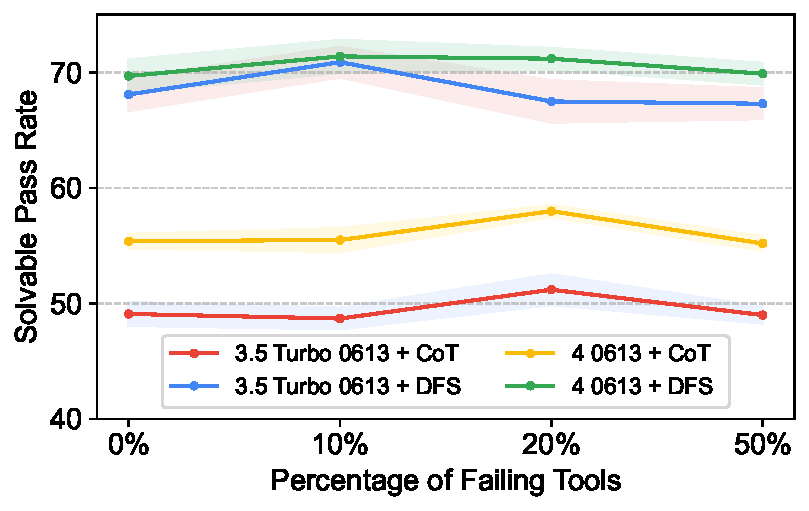
\includegraphics[width=\linewidth]{figs/virtual_solving_scores.pdf}
    \caption{Performance change when manually making APIs down with our virtual online API system. The results are averaged over all six groups. Solving rates are reported. We run each experiment one time and evaluate it three times and take the average score. Unless otherwise stated, \texttt{gpt-4-turbo-preview} at the time of testing is used in this section. This experiment was done in Feb 2024.}
    \label{fig:simulated_api_stability_test}
\end{figure}

Following the same setups as in \Cref{api_status}, we manually make the same success tools not available during the running time.
In our design, when a call is on an unavailable tool, it will be directed to the simulated API immediately.
Compared to \Cref{api_status}, the results as shown in \Cref{fig:simulated_api_stability_test} are much more stable with our virtual API server.
Even when 50\% of APIs are not available, changes in performance are still not significant, which is explainable within the range of variance.



% \textcolor{red}{change gpt-4 versions and other hyperparameters and run multiple sets of experiments. Aim to show change of GPT-4 won't affect the stability significantly.} 
Considering we use \texttt{gpt-4-turbo} as the backbone of the API simulator which may change even with the same version number, we ablate different versions and different temperatures of \texttt{gpt-4-turbo}.
The results are shown in \Cref{tab:server_config}.
Under different settings of the backbone LLMs, the performance change is still acceptable within the variance of LLM evaluation, indicating the robustness of our API simulators.



% \textcolor{red}{Discussion: An ultimate solution is to train a open-source models that make mock the API behavior well.
% }




% \begin{figure}
%     \centering
%     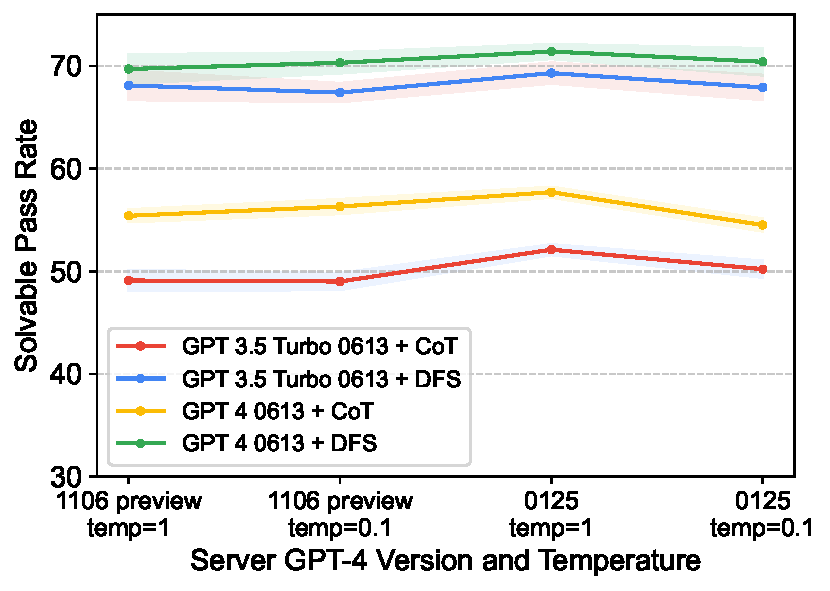
\includegraphics[width=\linewidth]{figs/virtual_solving_scores_against_server.pdf}
%     \caption{Performance of baselines with different settings of the LLM server. The results are averaged over all six groups. Solving rates are reported. We run each experiment one time and evaluate three times and take the average score.}
%     \label{fig:server_config}
% \end{figure}

\begin{table}
    \centering
    \small
    \resizebox{\linewidth}{!}{

    \begin{tabular}{lcccc}
        \toprule
        \multirow{2}{*}{\textbf{GPT-4 Config}} & \multicolumn{2}{c}{\textbf{1106-preview}} &  \multicolumn{2}{c}{\textbf{0125}} \\
        & \texttt{T=1} & \texttt{T=0.1} & \texttt{T=1} & \texttt{T=0.1}\\
        \midrule
         3.5 0613 (C) & 49.1{\tiny $\pm{1.0}$}  & 49.0{\tiny $\pm{0.8}$} & 52.1{\tiny $\pm{0.5}$} & 50.2{\tiny $\pm{0.8}$} \\
         3.5 0613 (D) & 68.1{\tiny $\pm{1.4}$}  & 67.4{\tiny $\pm{0.9}$} & 69.3{\tiny $\pm{1.0}$} & 67.9{\tiny $\pm{1.2}$}\\
         4 0613 (C) & 55.4{\tiny $\pm{0.6}$}  & 56.3{\tiny $\pm{0.7}$} & 57.7{\tiny $\pm{0.5}$} & 54.5{\tiny $\pm{0.6}$} \\
         4 0613 (D) & 69.7{\tiny $\pm{1.4}$}  & 70.3{\tiny $\pm{1.0}$} & 71.4{\tiny $\pm{0.7}$} & 70.4{\tiny $\pm{1.3}$}\\
         \midrule
         3.5 1106 (C) & 52.1{\tiny $\pm{0.7}$}  & 51.1{\tiny $\pm{0.5}$} & 54.5{\tiny $\pm{0.9}$} & 52.7{\tiny $\pm{0.6}$} \\
         3.5 1106 (D)  & 69.9{\tiny $\pm{0.7}$}  & 71.2{\tiny $\pm{0.9}$} & 70.0{\tiny $\pm{0.9}$} & 71.0{\tiny $\pm{0.9}$}\\
         4 Turbo (C) & 60.8{\tiny $\pm{0.7}$}  & 62.4{\tiny $\pm{0.8}$} & 63.6{\tiny $\pm{0.4}$} & 64.0{\tiny $\pm{1.1}$} \\
         4 Turbo (D) & 73.2{\tiny $\pm{1.1}$}  & 76.2{\tiny $\pm{0.9}$} & 75.0{\tiny $\pm{0.7}$} & 77.3{\tiny $\pm{0.9}$}\\     
        \bottomrule
    \end{tabular}
    }
    \caption{Performance of baselines with different settings of the LLM server. Results are averaged over all groups and reported in SoPR. We run each experiment one time and evaluate three times and take the average score.}
    \label{tab:server_config}
\end{table}

% Different models, same input, same outputs, temp=0




\subsection{Turing Test of API Simulator}
% \textcolor{red}{Aiming at testing the reality of APIs. 
% Sampling 100 API calls from real API responses and LLM faked responses, and ask GPT-4 / Human whether the two are indistinguishable (guess which is model and which is real). If the results are around 50\%. Then the test is passed.}
To test the effectiveness of API simulators, we design a ``Turing Test''~\cite{Turing2009} between the real APIs and the simulated ones.
% To successfully run experiments on a tool-learning benchmark, the fundamental requirement for the API system is that the responses of the API system are usable and believable by the testing model. 
% In this way, the testing model can use the outputs to finish an instruction. 
Note that we believe it is not required for API simulators to exactly output the same answers as those of real APIs, where rationality is more important.
% This is because the exact reality of API responses is not required for task completion.
For example, when a query asks about the weather today, the API simulator does not need to retrieve the ``real'' temperature. Instead, the API simulator needs to generate a reasonable temperature number.

To do the test, we first sample 70 available real APIs and their corresponding simulated APIs. 
% We then manually filter out unsuccessful real API calls, resulting in 70 API calls.
Given the API callings and their real and simulated response pairs, we ask three human annotators to determine which response more closely resembles an actual API response overall, based on the given descriptions of the API functions.
We ask human annotators to evaluate along three dimensions: Overall, Format Accuracy and Answer Relevance.
The annotator first need to answer which response is overall more like a real response.
When assessing format accuracy, annotators must determine which response more accurately adheres to the format specifications outlined in the documentation. In evaluating answer relevance, they are tasked with identifying which response more effectively fulfills the instruction in accordance with the documentation's guidelines.
The results are shown in ~\Cref{fig:turing_test}.
Surprisingly, human annotators cannot distinguish simulated and real APIs very well, where the simulated APIs are judged to act more like real situations.
Moreover, the proportion of tie is much larger, indicating that simulated APIs can work very similarly to real APIs.
% To further analyze the reason, we further ask human annotators to distinguish two kinds of APIs in terms of format accuracy and answer relevance only. As shown in \Cref{fig:turing_test}, one can see simulated APIs can work very similarly to the real APIs.


% \begin{table*}
%     \centering
%     \small
%     \begin{tabular}{cccccccccc}
%         \toprule
%         & \multicolumn{3}{c}{\textbf{Overall}} & \multicolumn{3}{c}{\textbf{Format Accuracy}}& \multicolumn{3}{c}{\textbf{Answer Relevance}}\\
%         \cmidrule(lr){2-4}
%         \cmidrule(lr){5-7}
%         \cmidrule(lr){8-10}
%         & {Real} &  {Simulated} & {Tie} & {Real} &  {Simulated} & {Tie}& {Real} &  {Simulated} & {Tie} \\
%         \midrule
%         % GPT-4-Turbo & 31.0 & 62.1 & 6.9 & 34.5 & 58.6 & 6.9 & 37.9 & 55.2 & 6.9  \\
%         % Gemini Pro & 31.0 & 69.0 & 0.0 & 20.7 & 79.3 & 0.0 & 31.0 & 65.5 & 3.4 \\
%         Human & 12.9\% & 20\% & 67.1\% & 0 \% & 5.7\% & 94.3\% & 10\% & 20\% & 70\% \\
%         \bottomrule
%     \end{tabular}
%     \caption{Results of the ``Turing Test'' for the real and LLM simulated APIs. \textcolor{red}{TODO: Change to bar figure.}}
%     \label{tab:turing_test}
% \end{table*}

\begin{figure}[t!]
    \centering
    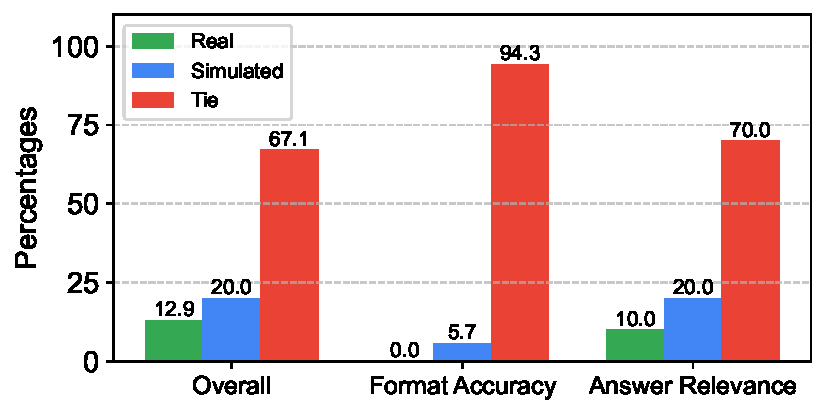
\includegraphics[width=\linewidth]{figs/turing_test.pdf}
    \caption{Results of the ``Turing Test'' for the real and simulated APIs. Results are win-lose-tie percentages.}
    \label{fig:turing_test}
\end{figure}

% We sample 50 LLM simulations from the Turing Test questions discussed in Section 4.3. Then we invite a human evaluator to answer whether the LLM simulation follows the documentation, i.e., whether it is a reasonable simulation that obeys the setting of the documentation. Results show that 90% of the simulations are deemed to be reasonable, 6% are not reasonable and 4% are not sure. It shows that the simulated APIs can well follow documentation.


In addition to the Turing Test mentioned above, we assess the quality of LLM simulations by evaluating the adherence of simulated outputs to their corresponding documentation. To conduct this evaluation, we randomly sample 50 simulated outputs along with their documentation from the Turing Test dataset. A human evaluator is then tasked with determining whether the LLM simulations reasonably follow the provided documentation. The results indicate that 90\% of the simulations are deemed reasonable, 6\% are considered unreasonable, and 4\% are uncertain. These findings suggest that the LLM is highly capable of generating simulated responses that adhere closely to the provided documentation.

% \begin{itemize}
%     \item Different inputs -> different outputs, same formats
% \end{itemize}


\subsection{Diversity of API Simulator}
% \textcolor{red}{Aim to show that API calls are diverse enough, so that the effective numbers of APIs won't decrease with simulated APIs.}
% \begin{enumerate}
%     \item Select a category of APIs, call these APIs in real and simulated ways. Calculate embeddings of these calls and see clustering outputs.
%     \item Call a selected APIs (potentially 10) with various arguments. See the difference across different arguments for both real and simulated APIs.
% \end{enumerate}
With the LLM simulation, API simulators will not exactly feedback the same as real APIs. 
Hence, a natural concern is whether the simulated APIs will degrade in diversity in API functionalities.
To study the problem, firstly, we explore the distribution of real and simulated API responses.
We first use all 246 APIs in the \texttt{Tool} API category from the successful APIs mentioned in \Cref{api_status}.
Then, we use the same call arguments to call these real and simulated APIs.
All the responses are encoded using S-BERT~\cite{reimers-2019-sentence-bert} and their corresponding embeddings are visualised by UMAP~\cite{mcinnes2018umap-software}. 
Detailed configuration is shown in \Cref{app:diversity_conf}.
The result is shown in \Cref{fig:diversity_comparison}. As can be seen from the figure, real and simulated APIs occupied similar embedding space, indicating that the diversity of simulated APIs is similar to the real APIs.

\begin{figure}[h!]
    \centering
    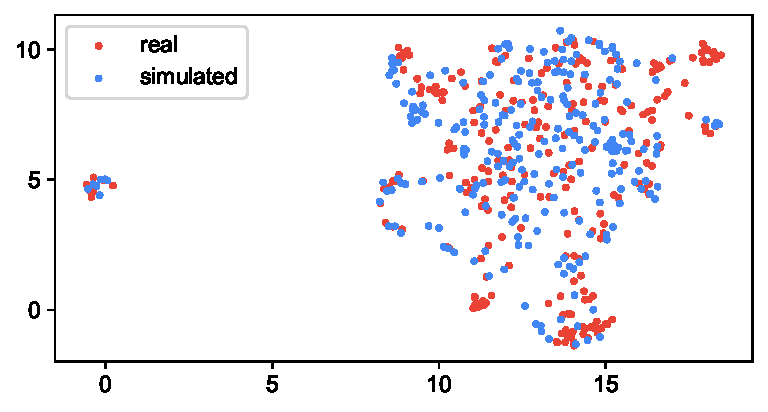
\includegraphics[width=\linewidth]{figs/diversity_comparison.pdf}
    \caption{Visualisation of the embeddings of responses from real and simulated APIs.}
    \label{fig:diversity_comparison}
\end{figure}

Secondly, we try to explore the behaviour when a simulated API is given several calls with different input arguments. 
We sample 60 APIs from all successful APIs and make 5 different calls to each API, using the same prompt as in \Cref{app:prompt_make_call}.
We then count the number of APIs that give exactly the same responses in any 2 of the 5 calls. Results show that only 2 of 60 APIs contain such responses, which supports the sufficient diversity of our simulated APIs.


\subsection{Effectiveness of Caching System}
% We run experiments on different methods and record the cache hit rate.
To show the effectiveness of our caching system in maintaining the stability of the virtual API server, we run several methods and record the cache hit rates. In detail, we run four methods used in ToolBench, \texttt{gpt-3.5-turbo-0613} and \texttt{gpt-4-0613} with CoT and DFS. Reproduction data in ToolBench of these methods has been used in the cache. Results are recorded in~\Cref{tab:cache_hit}, which shows that rerunning these in-domain methods has a very high cache hit rate. This means that most of the call responses are fixed and instability from the API system are much smaller. Nevertheless, models and methods may change over time, and therefore, we further run \texttt{gpt-3.5-turbo-1106} and \texttt{gpt-4-turbo-preview} with CoT and DFS.  As can be seen in the table, although the cache hit rates are smaller with these out-of-domain methods, the scores are still high enough to mitigate the instability significantly.



\subsection{Human Evaluation of Evaluator}
\label{sec:evaluator}

Considering that GPT-3.5 is limited to evaluating the performance in tool learning, we replace the automatic evaluators with stronger LLMs.
In this section, we manually assess the correctness of different automatic evaluators. 
Here, we sample 100 task-solvable questions, 50 answer-solving questions in the PR / SoPR evaluation, and 50 comparison questions in the WR / SoWR evaluation from the experiments running.

\begin{table}
    \centering
    \small
    \begin{tabular}{lccc}
        \toprule
        \textbf{Methods} & \textbf{Final} & \textbf{Mid} & \textbf{Start}\\
        \midrule
        GPT 3.5 Turbo 0613 + CoT & 96.7 & 36.2 & 11.7 \\
        GPT 3.5 Turbo 0613 + DFS & 97.0 & 34.5 & 11.6 \\
        GPT 4 0613 + CoT &  96.5 & 36.2 & 11.7\\
        GPT 4 0613  + DFS & 97.0 & 35.0 & 11.7 \\
         \midrule 
        GPT 3.5 Turbo 1106 + CoT & 91.4 & 35.1 & 11.8\\
         GPT 3.5 Turbo 1106 + DFS & 75.8 & 34.5 & 11.4 \\
        GPT 4 Turbo + CoT & 88.2 & 35.0 & 11.6 \\
        GPT 4 Turbo + DFS & 77.8 & 34.5 & 11.8\\
        \bottomrule
    \end{tabular}
    \caption{Cache hit rate (\%) with various models and methods. Final, Mid, and Start represent the final version of the cache, the mid-way version containing 151,152 (91.6\%) items of the final version, and the starting version containing only the train and test set. Experiments are independent runs of \Cref{sec:performance} with fixed cache, run on 13 Feb 2024.}
    \label{tab:cache_hit}
\end{table}
We then collect all the corresponding answers of different LLMs during previous evaluations.
% We use the same prompt and format as in the experiments. 
% We run \texttt{gpt-3.5-turbo}, \texttt{gpt-4-turbo}, \texttt{gemini-pro}, and \texttt{claude-2} on task solvable questions and \texttt{gpt-3.5-turbo}, \texttt{gpt-4-turbo} on answer solving and comparison questions.
These questions are further manually labeled by three human annotators to obtain the ground truth.
With the ground truth, we calculate the accuracy scores of these models and show the results in \Cref{tab:human_eval_task}. 
It can be seen that our used LLMs (i.e., Claude 2, Gemini, and GPT-4) are much better than GPT-3.5 in ToolBench to determine the solvability of tasks, where the Gemini and GPT-4 outperform by a large margin.
In both the evaluation of answers and comparison, GPT-4 significantly outperforms GPT-3.5, especially in the comparison to compute WR.
It is worth noting that all the accuracies of GPT-3.5 are lower than 70\%, indicating that GPT-3.5 cannot assess the performance in tool learning.
% \texttt{gemini-pro} and \texttt{claude-2} perform much better than \texttt{gpt-3.5-turbo} as well, which supports our model choices when judging task solvability above. 
% As a result, we replace {gpt-3.5-turbo} with \texttt{gpt-4-turbo} in the experiments below.



% \begin{table*}[]
%     \centering
%     \small
%     \begin{tabular}{cccccccc}
%         \toprule
%         \textbf{Method} &G1 Cat & G1 Inst & G1 Tool & G2 Cat & G2 Inst & G3 Inst & Avg \\
%         \midrule
%          ChatGPT + CoT & \\
%          ChatGPT + DFS \\
%          GPT-4 + CoT \\
%          GPT-4 + DFS \\
%          ToolLLaMA + CoT \\
%          ToolLLaMA + DFS \\
%          \bottomrule
%     \end{tabular}
%     \caption{NLI score}
%     \label{tab:my_label}
% \end{table*}




% \subsection{Human Evaluation on the NLI Metric}

% \section{Methods}
% \input{sections/3_methods}

% \section{Experiments}
% \input{sections/4_results}

% \section{Experiments}
% \subsection{Experimental Setups}

% \subsection{Query Construction}
% \textcolor{red}{Discussion: Position of query construction in the paper.}
% % Curating a large number of real-world queries based on a large-scale tool set is a non-trival problems. To balance 

% In addition to the original queries in ToolBench, we further create queries aiming at improved reality and quality of benchmark. In ToolBench, queries are created from the bottom-up, i.e., LLMs will write questions based on the APIs they are given. In this way, although the feasibility of the queries is guaranteed, reality is sacrificed. This is because when it comes to more complex multi-step questions, LLMs may connect unrelated APIs to make up an unnatural query. For example, in the following query: 

%  \texttt{I'm working on a project and I need some data related to addresses in Brazil. Can you provide me with address details using the postal code 75094080? Also, I would like to know the health status of the SQUAKE API.}

% \noindent The first and the second subquery, asking for address details and API status are not related.

% To enhance the reality of the queries, we further create some queries with cluster APIs functionalities with specified scenarios. Specifically, we first extract some scenarios from the training set of the ToolBench dataset, by prompting \texttt{GPT-4}. Then, we encode all tools by their documentation using \texttt{E5-Mistral-7B-Instruct}~\cite{wang2022text, wang2023improving}, following EasyTool~\cite{yuan2024easytool}. We cluster these APIs with K-Means~\cite{MacQueen1967SomeMF}. Within each cluster, we summarise the functionality of this cluster with \texttt{GPT-3.5-Turbo}. At last, for each scenario, we retrieve the top 5 clusters of APIs by the cosine similarity between the scenarios and the cluster centres and then ask GPT-4 to write queries based on the scenarios and retrieved clusters. Based on the clustered APIs, the detailed functionality of the APIs is blurred, allowing more natural queries.









% \section{Analysis}
% \subsection{Ablation studies}
\textcolor{red}{Analyse the impact of simulation and cache on the stability}

\section{Related Work}

\paragraph{Tool Learning Benchmarks.}
% \csj{please rewrite.}
Recent studies have shed light on the burgeoning capabilities of LLMs in understanding and mastering tools~\citep{li2023apibank, patil2023gorilla, gpt4tools, song2023restgpt, tang2023toolalpaca, ye2024tooleyes, xu2023tool}.
Gaining access to external tools endows LLMs with real-time factual knowledge~\citep{yang2023chatgpt}, multimodal functionalities~\citep{gupta2023visual}, and specialised skills in vertical domains~\citep{jin2023genegpt}. 
However, few work has been done to explore the stability of the tool environment in specific benchmarks and how it affects the LLMs' performance in tool-augmented tasks. 
% However, open-source LLMs still lag far behind the state-of-the-art LLMs in tool use, and how tool-use ability is acquired by SOTA LLMs remains unclear. In this paper, we aim to push the boundary by creating a stable tool-learning benchmark.

\paragraph{Tool Inference Methods.}
Recent literature has begun to explore various methodologies for integrating tool functionalities within LLMs. 
Notably, the robust in-context learning prowess of LLMs, as demonstrated in \cite{brown2020language}, has facilitated the augmentation of LLMs with external tools via in-context tool descriptions and demonstrations ~\citep{hsieh2023tool, ruan2023tptu, mialon2023augmented}.
An alternative approach involves the explicit training of LLMs ~\citep{patil2023gorilla, tang2023toolalpaca, chen2023fireact, qin2023toolllm, huang2023metatool} using datasets enriched with tool interactions, thereby familiarising models with the nuances of tool usage. 
% This area of research is pivotal, as it directly influences the efficiency and effectiveness of tool-augmented LLMs in performing a wide array of tasks.

\begin{table}[t!]
    \centering
    \small
    \begin{tabular}{lccc}
        \toprule
        \textbf{Methods} & \textbf{Solvability} &\textbf{Solving} & \textbf{Comparison} \\
        \midrule
         Claude 2 & 71.0 & - & -\\
         Gemini Pro & \textbf{82.0} & - & -\\
         GPT 3.5 Turbo & 65.0 & 68.0 & 56.0 \\
         GPT 4 Turbo & 80.0 & \textbf{74.0} & \textbf{78.0}\\
         
         
         \bottomrule
    \end{tabular}
    \caption{Human evaluation on task solvability, answer solving (for pass rate) and comparison (for win rate).}
    \label{tab:human_eval_task}
\end{table}

\paragraph{Evaluation in Tool Learning.}
Evaluating the performance of LLMs in tool-augmented tasks presents unique challenges and opportunities.
Numerous works have been developed for the assessment of tool utilisation, primarily emphasising response comparison ~\citep{zhuang2023toolqa}, tool call accuracy ~\citep{patil2023gorilla}, or a synthesis of these aspects ~\citep{li2023apibank}. Distinguishing itself, \cite{qin2023toolllm} introduces an innovative methodology by integrating a large language model (LLM) as a judge to evaluate the comprehensive solution path. 
Subsequent research ~\citep{wang2023mint} focuses on the multi-turn interaction capabilities of LLMs with both tools and user feedback.
In a departure from the aforementioned approaches, \cite{chen2023teval} presents itself as the inaugural benchmark specifically tailored for the fine-grained assessment of tool utilisation capabilities.
% These evaluation methodologies offer insights into the effectiveness of LLMs in real-world scenarios, highlighting areas for further improvement and refinement. 
However, there exists a gap in the literature concerning the exploration of evaluation stability when evaluating the tool usage capabilities of LLMs.

% \paragraph{In-context Learning with LLMs.}
% % for response generation
% In-context learning has been a transformative technique enabling LLMs to perform a wide range of tasks without fine-tuning. \cite{radford2019language} introduced the GPT series, demonstrating the potential of transformer-based models for in-context learning across various natural language processing tasks. \cite{brown2020language} furthered this work with GPT-3, showcasing the ability of LLMs to perform tasks given a small number of examples, or even a single example, within the prompt. This capability forms the foundation of our approach to mimicking API behavior.

% \paragraph{Instruction Generation.}
% The evolution of LLMs has enabled not only the comprehension but also the generation of instructions, marking a significant leap in natural language understanding and generation. 
% Benchmarks and tasks designed around instruction generation, as proposed by \citet{wei2021finetuned} and \citet{mishra2021cross}, demonstrate the potential of LLMs to craft coherent and contextually relevant instructions. 
% Following works ~\citep{patil2023gorilla, qin2023toolllm, tang2023toolalpaca} directly prompt LLMs to generate high-quality instructions or user queries under tool learning scenarios, demonstrating the effectiveness of utilizing LLMs for real-world instruction generation.

% \paragraph{API Generation and Simulation.}




% \section{Discussion}
% The phenomenon may occur beyound tool learning
% The experiments can be put afterwards, Stability first

\section{Conclusion}
% In this paper, to improve the stability of ToolBench, we propose a new stable benchmark named StableToolBench. Starting by the analysis of ToolBench, we find that the original ToolBench suffers from instability of evaluation processes and API status, which leads to fluctuation of evaluated model performance. To tackle the problem, we firstly determined all solvable problems in advance. We then replace the real API server with a virtual API server, supported by GPT-4 simulation of API behaviours when real APIs are not available. Finally, we build a caching system to store the server responses to use for increased stability. Extensive experiments show that StableToolBench can provide much more stable model performance. The simulated APIs demonstrate considerable reality and diversity while the caching system plays an important role in increasing stability.

In this paper, we propose StableToolBench, a benchmark developed to enhance the stability of ToolBench. Our analysis identified instability issues in the evaluation processes of ToolBench and API status, causing variability in model performance assessments. To address this, we implement a caching system for consistent data availability. We also replace the real API server with an LLM-simulated virtual server for reliable API behaviour simulation. Experiments show that StableToolBench significantly improves the stability of model performance evaluations, with the simulated APIs offering realism and the caching system contributing greatly to the enhanced stability of the benchmark.

% \clearpage
\section*{Acknowledgement}
This work is supported by the National Natural Science Foundation of China (No. 62276152, 61925601).
We also extend our gratitude to Jingwen Wu and Yao Li for their assistance with human evaluation and additional suggestions.
 
\section*{Limitations}
In this work, we propose StableToolBench, a new tool learning benchmark with increased stability but non-declining reality. However, our work faces the following limitations. Firstly, we used GPT-4 as the automatic evaluator in the evaluation process and as the backbone server, which increase the cost of using our benchmark. 
% Secondly, despite careful designs, including fixed version number and other parameters, GPT-4 as an backbone server still suffers from subtle instability when OpenAI updates its model. Though the impact of such instability is limited, we aim to further improve it by training an open-source model in the future. 
Secondly, the GPT-4 backboned server demonstrate strong performance in simulating API behaviours. Nevertheless, the backbone LLM may experience significant upgrades, which may affect the performance.
Therefore, we believe that the ultimate solution is to solve the problem with a trained open-source LLM. However, current open-source LLMs are not performant enough to simulate API behaviours well. As a result, closed-source LLMs are the only options. 
We believe that when open-source LLMs are strong enough to be well suited for this task, 
In the future, we may turn to open-source LLMs when they are strong enough to be well suited for this task.
Thirdly, although the cache hit rates are high with our explored methods, new methods will be developed in the future. Whether this cache will still be effective is unsure. In this regard, we aim to continuously update the cache in the future in a slow pace for both balanced stability and effectiveness. 


% Nevertheless, the backbone LLM may experience significant upgrades, which may affect the performance.
% Therefore, we believe that the ultimate solution is to solve the problem with a trained open-source LLM. However, current open-source LLMs are not performant enough to simulate API behaviours well. As a result, closed-source LLMs are the only options. 
% % We believe that when open-source LLMs are strong enough to be well suited for this task, 
% In the future, we may turn to open-source LLMs when they are strong enough to be well suited for this task.

\bibliography{custom}

\clearpage
\appendix
\section{Additional Results}
\subsection{GPT-3 Experiments} 
\label{sec:gpt3}
\begin{table}[ht]
    \centering
\begin{tabular}{c | cc}
\toprule
 & PaLM-540B & GPT-3 \\ \midrule
HotpotQA (exact match) & 29.4 & \textbf{30.8} \\
ALFWorld (success rate \%) & 70.9 & \textbf{78.4} \\ 
\bottomrule
\end{tabular}%
    \caption{\model{} prompting results using PaLM-540B vs.\,GPT-3 (text-davinci-002, greedy decoding). On HotpotQA, we randomly sample a subset of 500 validation questions. On ALFWorld, we use all 134 unseen validation task instances, and use the best prompt set according to PaLM-540B.}
    \label{tab:gpt3}
\end{table}
We run additional GPT-3~\citep{brown2020language} experiments to confirm \model{} prompting performance is general across different large language models. As shown in Table~\ref{tab:gpt3}, GPT-3 (text-davinci-002, greedy decoding) consistently outperforms PaLM-540B on HotpotQA and ALFWorld, possibly because it is finetuned with human instruction following. This indicates ReAct prompting is effective across different large language models on different tasks.
The code for these experiments are at \url{https://react-lm.github.io/}.
\subsection{\model{} obtains up-to-date knowledge on HotpotQA}
\begin{figure}[ht]
    \centering
    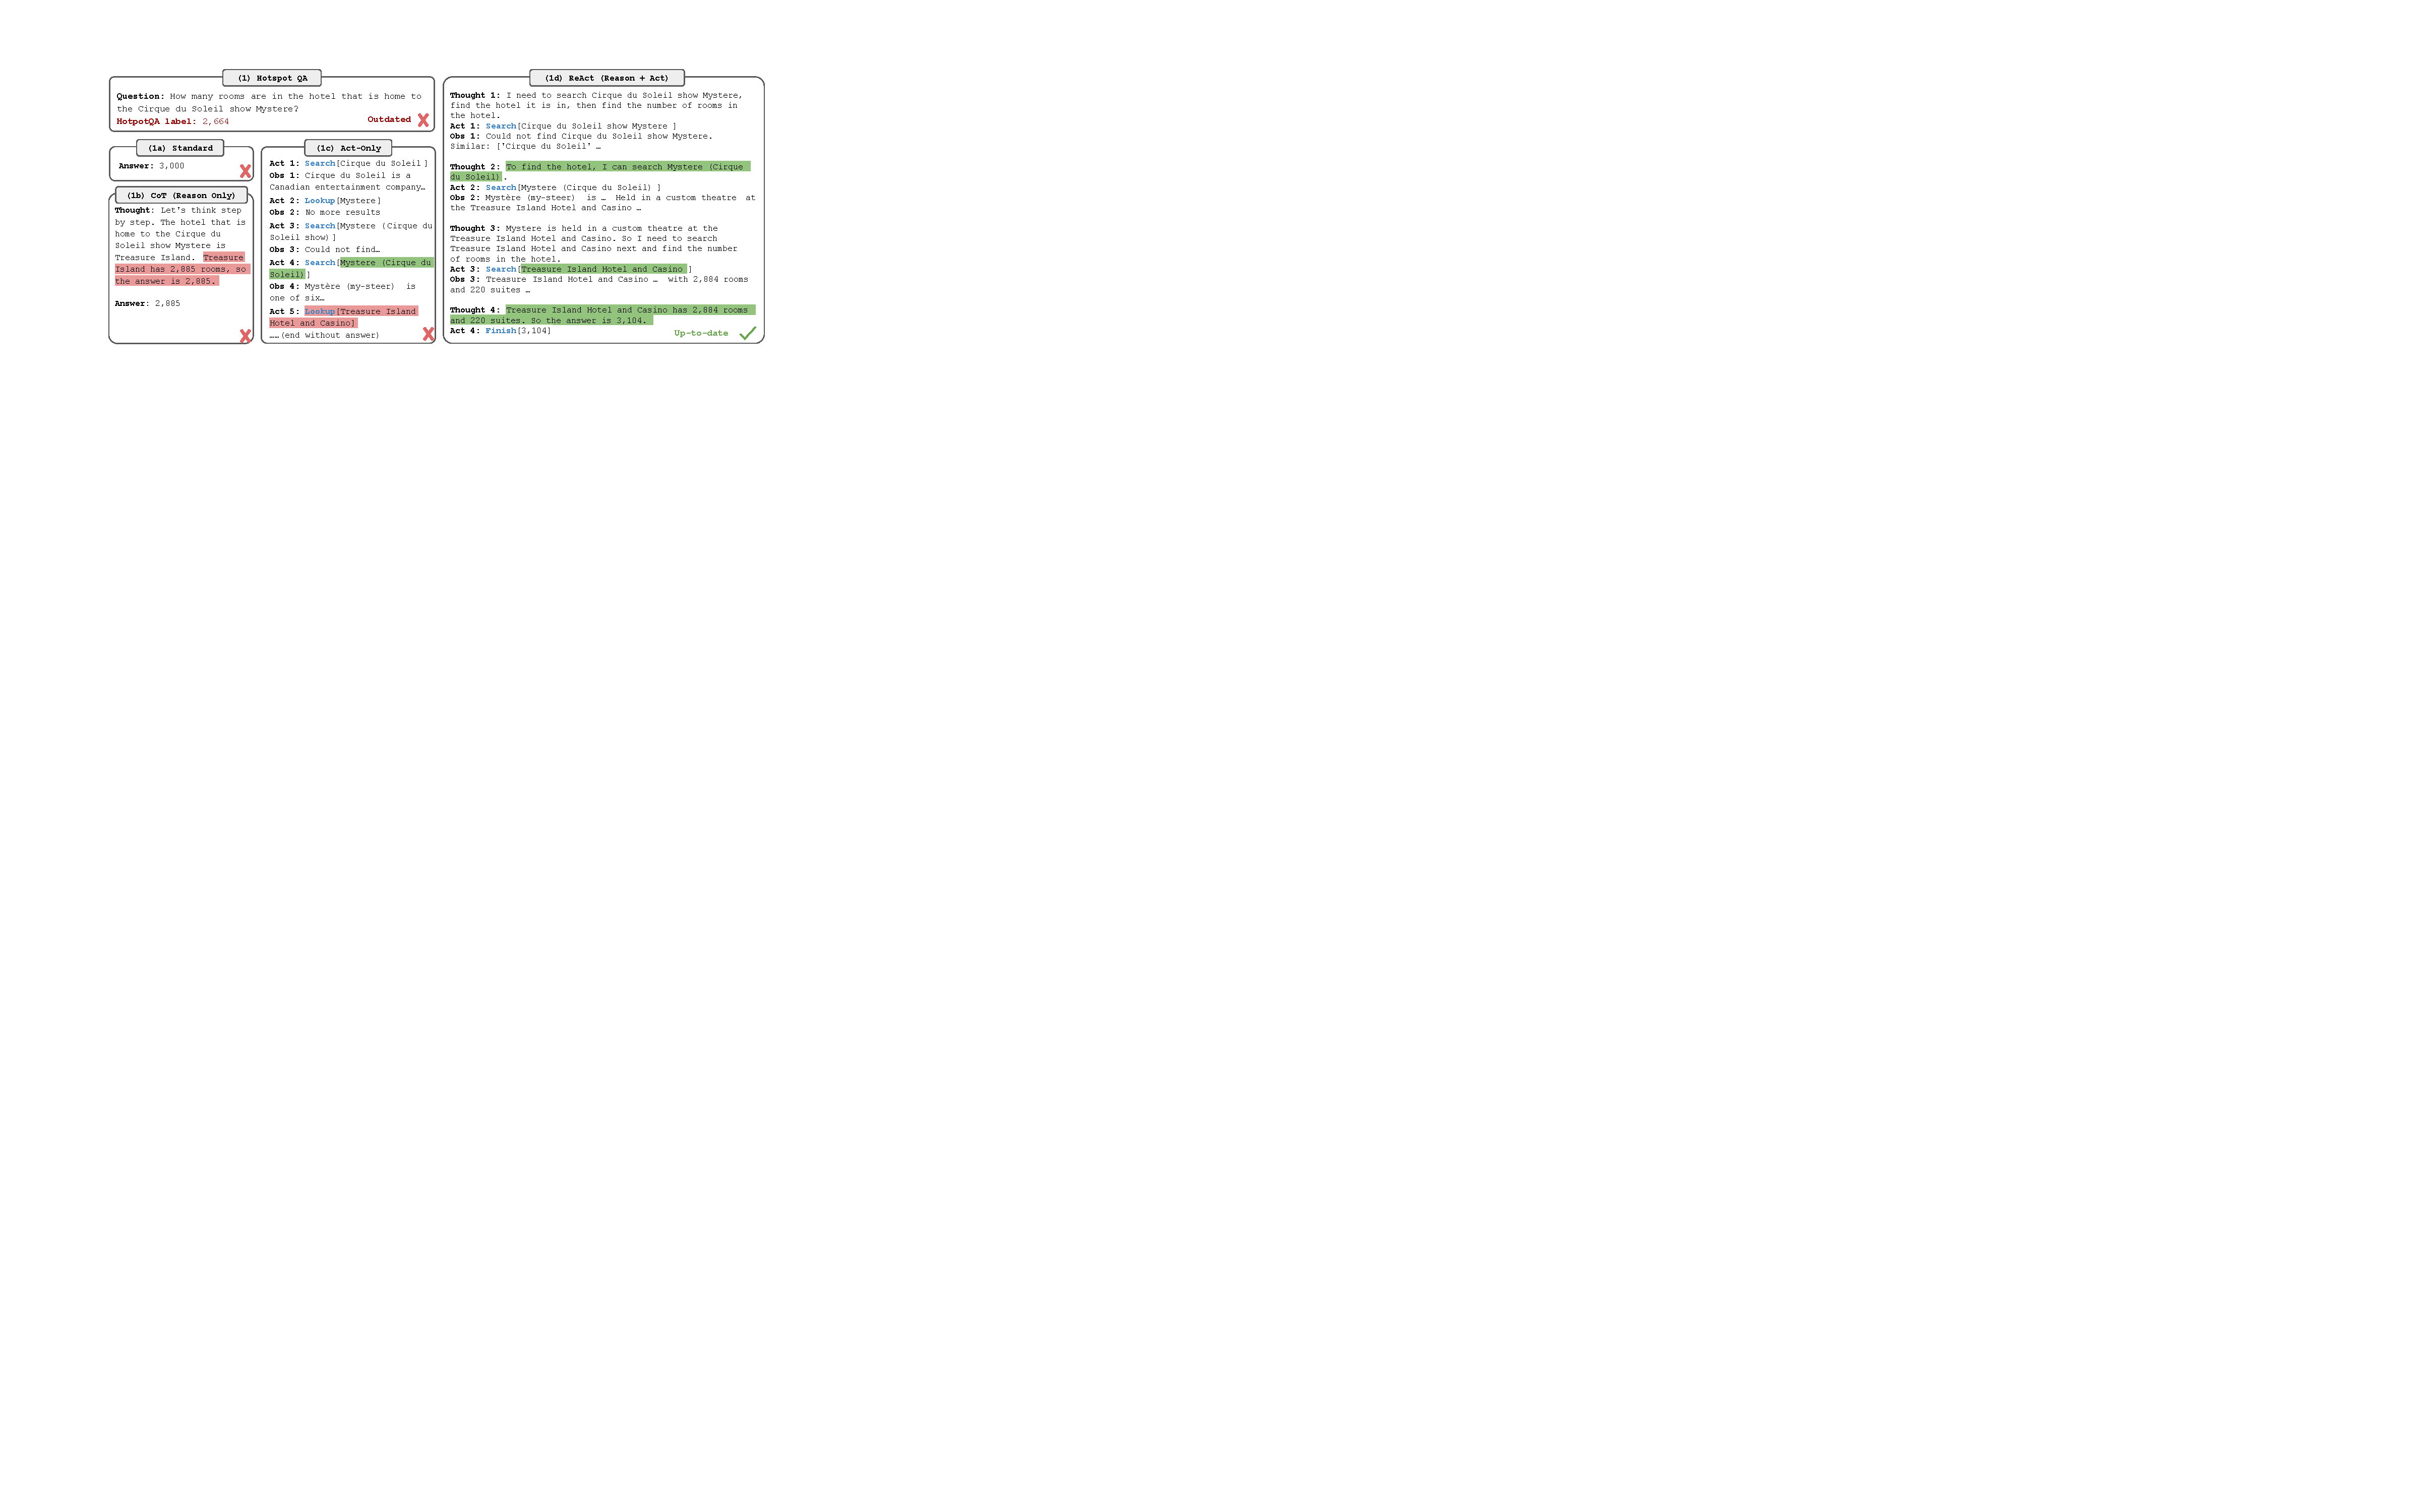
\includegraphics[width=\textwidth]{iclr2023/figure/date.pdf}
    \caption{
    {
    Another example HotpotQA question, where the original label is outdated. Only \model{} is able to obtain the up-to-date answer thanks to real-world web interaction plus reasoning.}
    }
    \label{fig:date}
    \vspace{-10pt}
\end{figure}

During trajectory inspection, we also find that sometimes \model{} does not agree with dataset labels as the labels themselves could be outdated. For example, as shown in Figure~\ref{fig:date}, the question asks about the size of a hotel, which increased from the HotpotQA construction time. While \palm{} and \reason{} give wrong answers due to hallucination, \act{} fails despite the access of real-world web interaction, due to a lack of reasoning to guide how to interact with the Internet for QA. Only \model{} is able to retrieve up-to-date information from the Internet and provide a reasonable answer. Therefore, better incorporation of reasoning abilities might benefit recent Internet-augmented language models~\citep{nakano2021webgpt,lazaridou2022internet,shuster2022language} for up-to-date task solving. 
\subsection{Human-in-the-loop behavior correction on AlfWorld} 
\begin{figure}[ht]
    \centering
    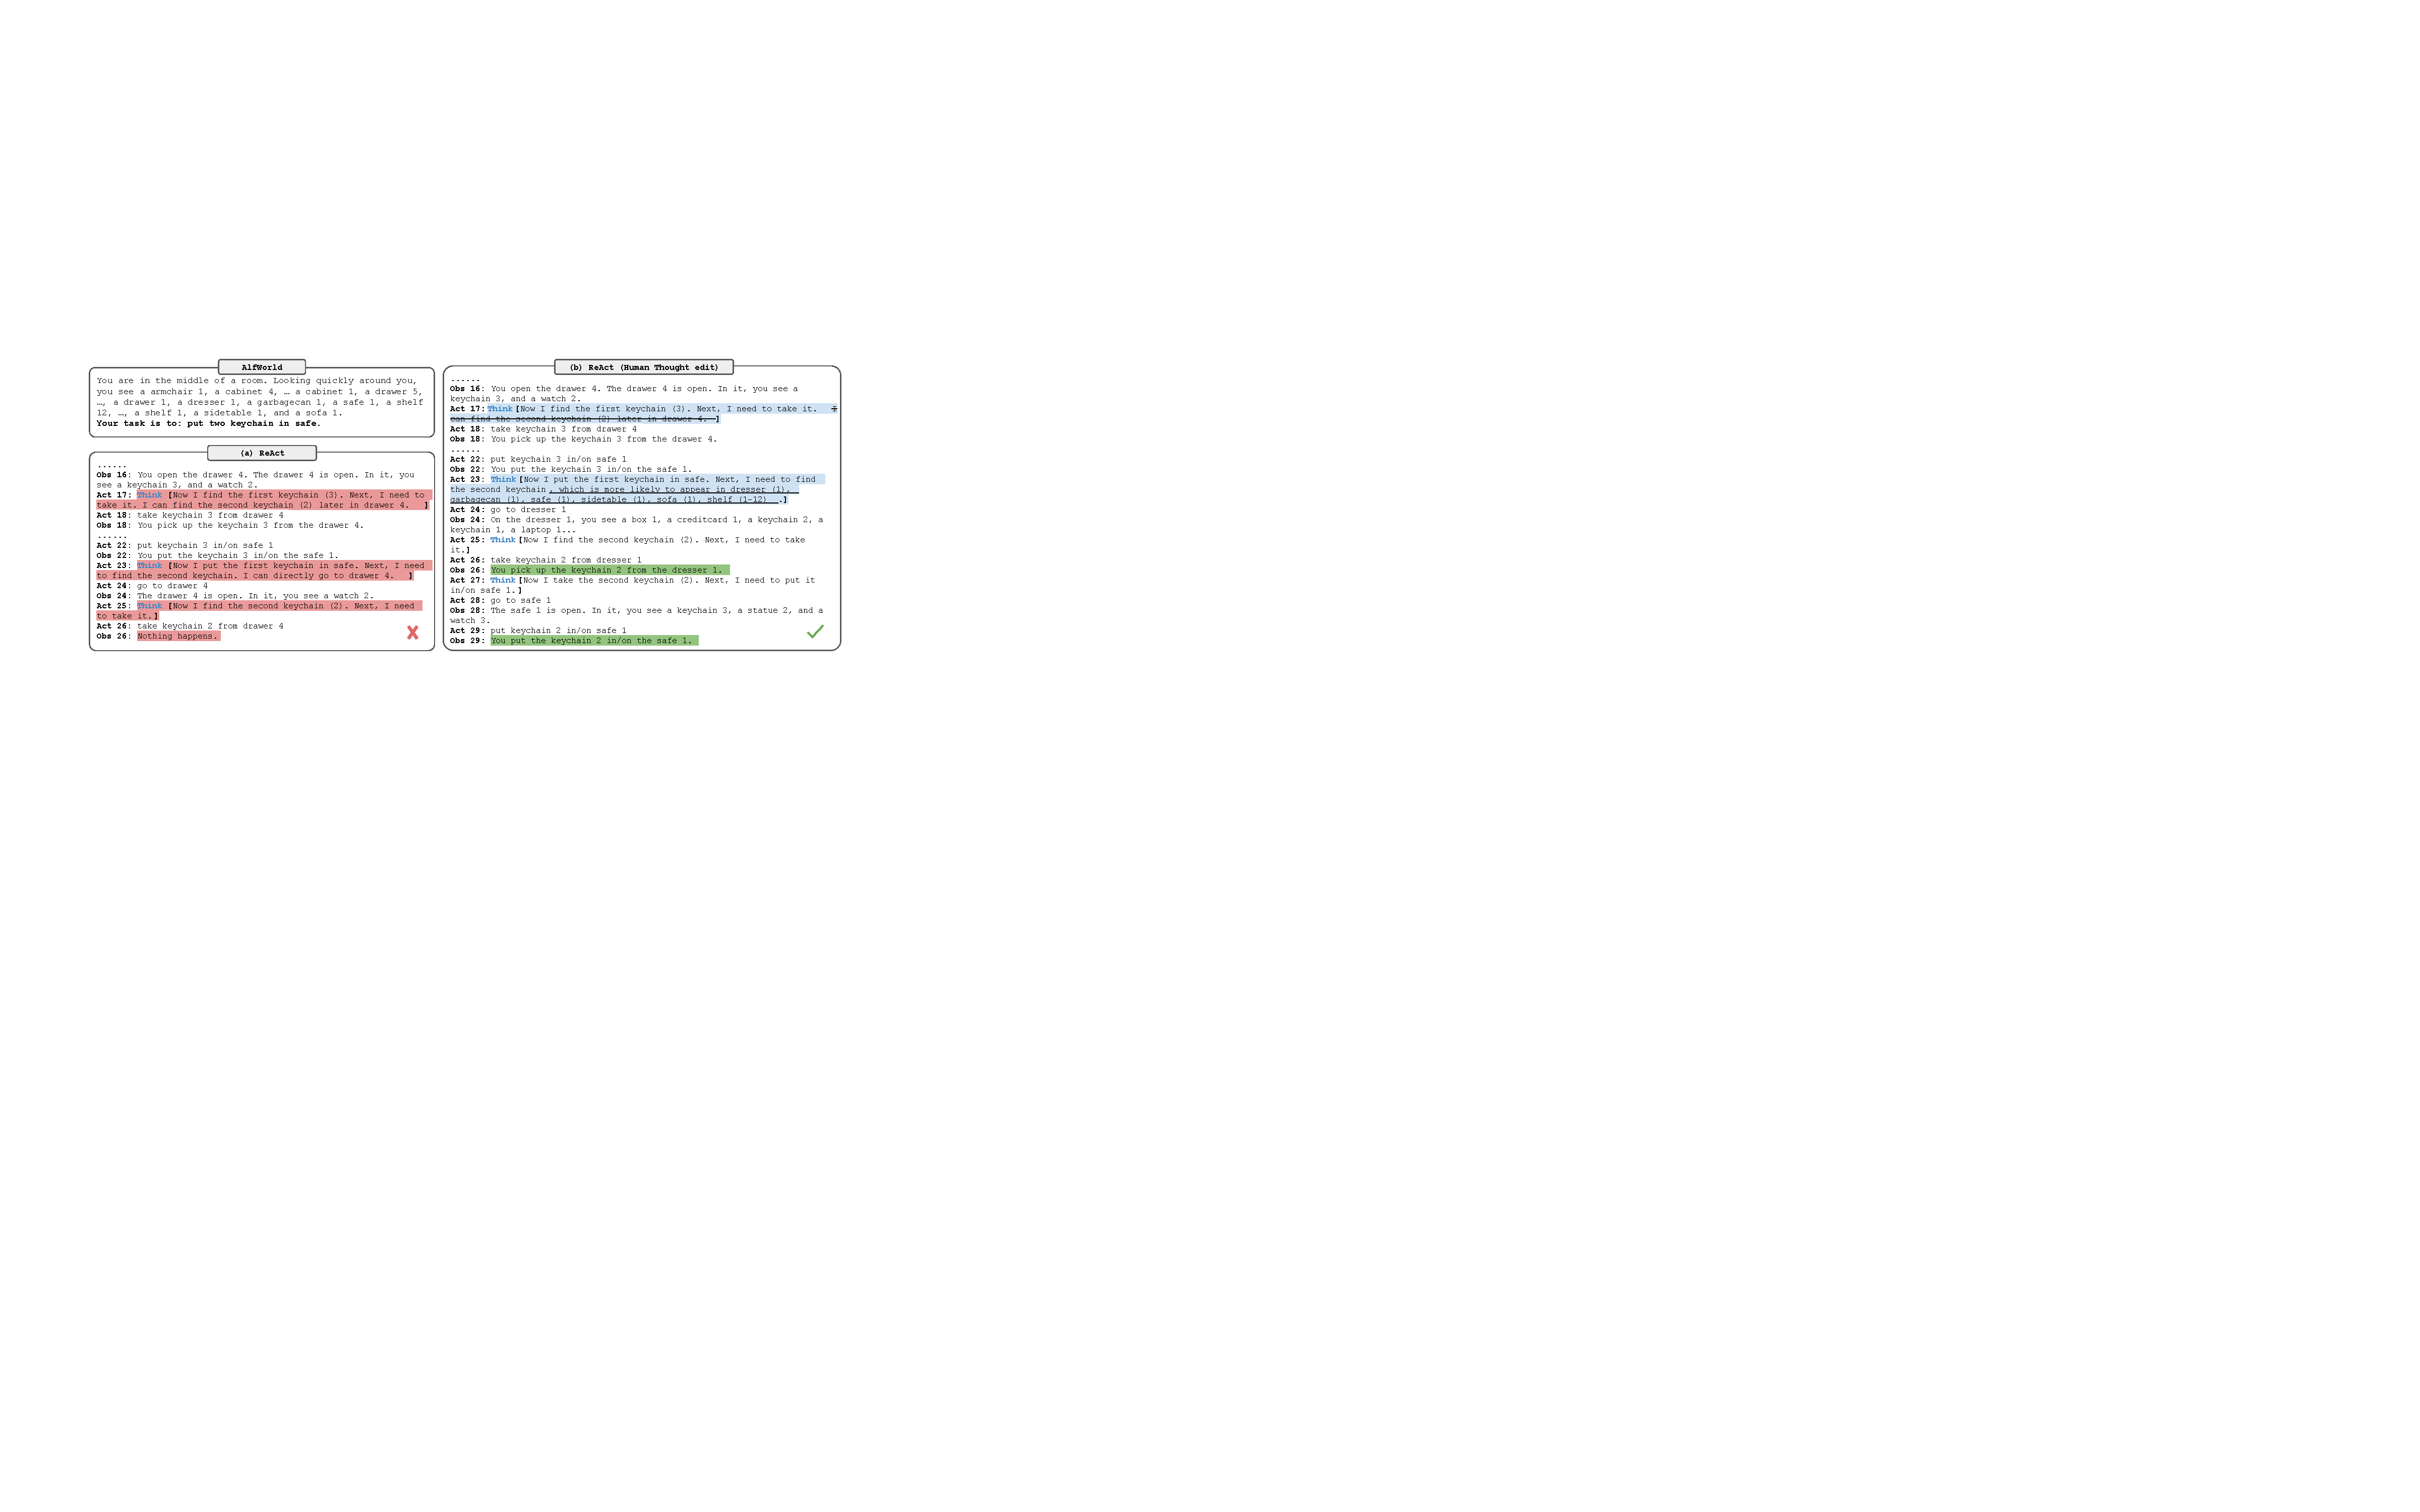
\includegraphics[width=\textwidth]{iclr2023/figure/human_edit.pdf}
    \caption{
    A human-in-the-loop behavior correction example with \model{} in AlfWorld. 
    (a) \model{} trajectory fails due to a hallucinating thought (Act 17).
    (b) By a human simply editing two thoughts (Act 17, 23), the \model{} trajectory produces desirable reasoning traces and actions and succeeds.
    }
    \label{fig:edit}
    \vspace{-10pt}
\end{figure}

We also explore human-in-the-loop interaction with \model{}, to allow a human to inspect and edit \model's reasoning traces. Figure~\ref{fig:edit} shows that
by simply removing a hallucinating sentence in Act 17 and adding some hints in Act 23, \model{} can be made to change its behavior drastically to align with these human thought edits and succeed in the task. 
From a human perspective, solving such a task becomes significantly easier, from typing tens of actions to only editing a couple of thoughts, which enables new forms of human-machine collaboration.
We note that such a policy edit on-the-go is difficult for \act{} and previous RL methods, as a human cannot change the model parameters, and changing a few actions might not edit the rest of the model behavior. 
This paradigm is also more than human dialogue to update the goal or subgoal as in \citet{huang2022inner} --- while editing \model{} thoughts can do these, it can also modify the model's internal belief, reasoning styles, or anything the flexible thought space supports, for better task solving. 
We believe this is an exciting direction for human alignment and leave more systematic study as future work.

\section{Experiment Details}
\subsection{HotpotQA Finetuning Details}
\label{sec:hotpot_finetune}
For all finetuning we use a batch size of 64.
On PaLM-8B, we finetune \model{} and \act{} methods for $4,000$ steps and \palm{} and \reason{} methods for $2,000$ steps. 
On PaLM-62B, we finetune \model{} and \act{} methods for $4,000$ steps and \palm{} and \reason{} methods for $1,000$ steps. 
We find \model{} and \act{} methods generally benefit from more training steps (and more training data), while  \palm{} and \reason{} methods degrade soon after finetuning.

\subsection{AlfWorld IM-Style Details}
\label{sec:alfworld_im}
For the IM-style ablation, the same expert trajectories used in \model{} are reannotated with dense external feedback thoughts within these trajectories, that limit \modelim{} to only think about (1) decomposing the current goal and (2) the current subgoal that needs to be completed. In particular, \modelim{} lacks thoughts that (1) determine when a subgoal is completed (2) determine what the next subgoal should be (3) inducing the LLM to refer to its internal pretraining knowledge to identify where items can be within the environment. 


\section{Prompts}
\label{sec:prompts}
\subsection{HotpotQA}
\begin{table}[H]
\scriptsize
\begin{minipage}{0.9\linewidth}
Hotpot QA Prompts
\centering
\ttfamily
\begin{tabular}{l p{0.9\linewidth}}
\midrule
\sethlcolor{cyan}\hl{Original} & \\
Question &  What is the elevation range for the area that the eastern sector of the Colorado orogeny extends into? \\
Answer &  1,800 to 7,000 ft\\
\\
Question &  Musician and satirist Allie Goertz wrote a song about the "The Simpsons" character Milhouse, who Matt Groening named after who?\\
Answer &  Richard Nixon\\
\\
Question &  Which documentary is about Finnish rock groups, Adam Clayton Powell or The Saimaa Gesture?\\
Answer &  The Saimaa Gesture\\
\\
Question &  What profession does Nicholas Ray and Elia Kazan have in common?\\
Answer &  director, screenwriter, actor\\
\\
Question &  Which magazine was started first Arthur's Magazine or First for Women?\\
Answer &  Arthur's Magazine\\
\\
Question &  Were Pavel Urysohn and Leonid Levin known for the same type of work?\\
Answer &  Yes\\


\midrule
\sethlcolor{red}\hl{\act} & \\
Question &  What is the elevation range for the area that the eastern sector of the Colorado orogeny extends into?\\
Action 1 &  Search[Colorado orogeny]\\
Observation 1 &  The Colorado orogeny was an episode of mountain building (an orogeny) in Colorado and surrounding areas.\\
Action 2 &  Lookup[eastern sector]\\
Observation 2 &  (Result 1 / 1) The eastern sector extends into the High Plains and is called the Central Plains orogeny.\\
Action 3 &  Search[High Plains]\\
Observation 3 &  High Plains refers to one of two distinct land regions: \\
Action 4 &  Search[High Plains (United States)]\\
Observation 4 &  The High Plains are a subregion of the Great Plains. From east to west, the High Plains rise in elevation from around 1,800 to 7,000 ft (550 to 2,130 m).[3]\\
Action 5 &  Finish[1,800 to 7,000 ft]\\
\\
Question &  Musician and satirist Allie Goertz wrote a song about the "The Simpsons" character Milhouse, who Matt Groening named after who?\\
Action 1 &  Search[Milhouse]\\
Observation 1 &  Milhouse Mussolini Van Houten is a recurring character in the Fox animated television series The Simpsons voiced by Pamela Hayden and created by Matt Groening.\\
Action 2 &  Lookup[named after]\\
Observation 2 &  (Result 1 / 1) Milhouse was named after U.S. president Richard Nixon, whose middle name was Milhous. \\
Action 3 &  Finish[Richard Nixon]\\
\\
Question &  Which documentary is about Finnish rock groups, Adam Clayton Powell or The Saimaa Gesture?\\
Action 1 &  Search[Adam Clayton Powell]\\
Observation 1 &  Could not find [Adam Clayton Powell]. Similar:  ['Adam Clayton Powell III', 'Seventh Avenue (Manhattan)', 'Adam Clayton Powell Jr. State Office Building', 'Isabel Washington Powell', 'Adam Powell', 'Adam Clayton Powell (film)', 'Giancarlo Esposito'].\\
Action 2 &  Search[Adam Clayton Powell (film)]\\
Observation 2 &  Adam Clayton Powell is a 1989 American documentary film directed by Richard Kilberg. The film is about the rise and fall of influential African-American politician Adam Clayton Powell Jr.[3][4] It was later aired as part of the PBS series The American Experience.\\
Action 3 &  Finish[The Saimaa Gesture]\\
\\
Question &  What profession does Nicholas Ray and Elia Kazan have in common?\\
Action 1 &  Search[Nicholas Ray]\\
Observation 1 &  Nicholas Ray (born Raymond Nicholas Kienzle Jr., August 7, 1911 – June 16, 1979) was an American film director, screenwriter, and actor best known for the 1955 film Rebel Without a Cause.\\
Action 2 &  Search[Elia Kazan]\\
Observation 2 &  Elia Kazan was an American film and theatre director, producer, screenwriter and actor.\\


\midrule \multicolumn{2}{r}{\textit{Continued on next page}} \\
\end{tabular}
\end{minipage}%
\end{table}


\begin{table}[H]
\scriptsize
\begin{minipage}{0.9\linewidth}
Hotpot QA Prompts -- Continued from previous page
\centering
\ttfamily
\begin{tabular}{l p{0.9\linewidth}}
\midrule
\\
Action 3 &  Finish[director, screenwriter, actor]\\
Question &  Which magazine was started first Arthur's Magazine or First for Women?\\
Action 1 &  Search[Arthur's Magazine]\\
Observation 1 &  Arthur's Magazine (1844--1846) was an American literary periodical published in Philadelphia in the 19th century. \\
Action 2 &  Search[First for Women]\\
Observation 2 &  First for Women is a woman's magazine published by Bauer Media Group in the USA.[1] The magazine was started in 1989. \\
Action 3 &  Finish[Arthur's Magazine]\\
\\
Question &  Were Pavel Urysohn and Leonid Levin known for the same type of work?\\
Action 1 &  Search[Pavel Urysohn]\\
Observation 1 &  Pavel Samuilovich Urysohn (February 3, 1898 - August 17, 1924) was a Soviet mathematician who is best known for his contributions in dimension theory.\\
Action 2 &  Search[Leonid Levin]\\
Observation 2 &  Leonid Anatolievich Levin is a Soviet-American mathematician and computer scientist. \\
Action 3 &  Finish[yes]\\
\midrule
\sethlcolor{green}\hl{\reason} & \\
Question &  What is the elevation range for the area that the eastern sector of the Colorado orogeny extends into?\\
Thought &  Let's think step by step. The eastern sector of Colorado orogeny extends into the High Plains. High Plains rise in elevation from around 1,800 to 7,000 ft, so the answer is 1,800 to 7,000 ft.\\
Answer &  1,800 to 7,000 ft\\
\\
Question &  Musician and satirist Allie Goertz wrote a song about the "The Simpsons" character Milhouse, who Matt Groening named after who?\\
Thought &  Let's think step by step. Milhouse was named after U.S. president Richard Nixon, so the answer is Richard Nixon.\\
Answer &  Richard Nixon\\
\\
Question &  Which documentary is about Finnish rock groups, Adam Clayton Powell or The Saimaa Gesture?\\
Thought &  Let's think step by step. Adam Clayton Powell (film) is a documentary about an African-American politician, not Finnish rock groups. So the documentary about Finnish rock groups must instead be The Saimaa Gesture.\\
Answer &  The Saimaa Gesture\\
\\
Question &  What profession does Nicholas Ray and Elia Kazan have in common?\\
Thought &  Let's think step by step. Professions of Nicholas Ray are director, screenwriter, and actor. Professions of Elia Kazan are director, producer, screenwriter, and actor. So profession Nicholas Ray and Elia Kazan have in common is director, screenwriter, and actor.\\
Answer &  director, screenwriter, actor\\
\\
Question &  Which magazine was started first Arthur's Magazine or First for Women?\\
Thought &  Let's think step by step. Arthur's Magazine was started in 1844. First for Women was started in 1989. 1844 (Arthur's Magazine) < 1989 (First for Women), so Arthur's Magazine was started first.\\
Answer &  Arthur's Magazine\\
\\
Question &  Were Pavel Urysohn and Leonid Levin known for the same type of work?\\
Thought &  Let's think step by step. Pavel Urysohn is a mathematician. Leonid Levin is a mathematician and computer scientist. So Pavel Urysohn and Leonid Levin have the same type of work.\\
Answer &  Yes\\


\midrule
\sethlcolor{yellow}\hl{\model} & \\
Question &  What is the elevation range for the area that the eastern sector of the Colorado orogeny extends into?\\
Thought 1 &  I need to search Colorado orogeny, find the area that the eastern sector of the Colorado orogeny extends into, then find the elevation range of the area.\\
Action 1 &  Search[Colorado orogeny]\\
Observation 1 &  The Colorado orogeny was an episode of mountain building (an orogeny) in Colorado and surrounding areas.\\
Thought 2 &  It does not mention the eastern sector. So I need to look up eastern sector.\\
Action 2 &  Lookup[eastern sector]\\
Observation 2 &  (Result 1 / 1) The eastern sector extends into the High Plains and is called the Central Plains orogeny.\\
Thought 3 &  The eastern sector of Colorado orogeny extends into the High Plains. So I need to search High Plains and find its elevation range.\\
Action 3 &  Search[High Plains]\\
Observation 3 &  High Plains refers to one of two distinct land regions  \\
Thought 4 &  I need to instead search High Plains (United States).\\
Action 4 &  Search[High Plains (United States)]\\

\midrule \multicolumn{2}{r}{\textit{Continued on next page}} \\

\end{tabular}
\end{minipage}%
\end{table}


\begin{table}[H]
\scriptsize
\begin{minipage}{0.9\linewidth}
Hotpot QA Prompts -- Continued from previous page
\centering
\ttfamily
\begin{tabular}{l p{0.9\linewidth}}
\midrule
\\
Observation 4 &  The High Plains are a subregion of the Great Plains. From east to west, the High Plains rise in elevation from around 1,800 to 7,000 ft (550 to 2,130 m).[3]\\
Thought 5 &  High Plains rise in elevation from around 1,800 to 7,000 ft, so the answer is 1,800 to 7,000 ft.\\
Action 5 &  Finish[1,800 to 7,000 ft]\\
\\
Question &  Musician and satirist Allie Goertz wrote a song about the "The Simpsons" character Milhouse, who Matt Groening named after who?\\
Thought 1 &  The question simplifies to "The Simpsons" character Milhouse is named after who. I only need to search Milhouse and find who it is named after.\\
Action 1 &  Search[Milhouse]\\
Observation 1 &  Milhouse Mussolini Van Houten is a recurring character in the Fox animated television series The Simpsons voiced by Pamela Hayden and created by Matt Groening.\\
Thought 2 &  The paragraph does not tell who Milhouse is named after, maybe I can look up "named after".\\
Action 2 &  Lookup[named after]\\
Observation 2 &  (Result 1 / 1) Milhouse was named after U.S. president Richard Nixon, whose middle name was Milhous. \\
Thought 3 &  Milhouse was named after U.S. president Richard Nixon, so the answer is Richard Nixon.\\
Action 3 &  Finish[Richard Nixon]\\
\\
Question &  Which documentary is about Finnish rock groups, Adam Clayton Powell or The Saimaa Gesture?\\
Thought 1 &  I need to search Adam Clayton Powell and The Saimaa Gesture, and find which documentary is about Finnish rock groups.\\
Action 1 &  Search[Adam Clayton Powell]\\
Observation 1 &  Could not find [Adam Clayton Powell]. Similar:  ['Adam Clayton Powell III', 'Seventh Avenue (Manhattan)', 'Adam Clayton Powell Jr. State Office Building', 'Isabel Washington Powell', 'Adam Powell', 'Adam Clayton Powell (film)', 'Giancarlo Esposito'].\\
Thought 2 &  To find the documentary, I can search Adam Clayton Powell (film).\\
Action 2 &  Search[Adam Clayton Powell (film)]\\
Observation 2 &  Adam Clayton Powell is a 1989 American documentary film directed by Richard Kilberg.
The film is about the rise and fall of influential African-American politician Adam Clayton Powell Jr.[3][4] It was later aired as part of the PBS series The American Experience.\\
Thought 3 &  Adam Clayton Powell (film) is a documentary about an African-American politician, not Finnish rock groups. So the documentary about Finnish rock groups must instead be The Saimaa Gesture.\\
Action 3 &  Finish[The Saimaa Gesture]\\
\\
Question &  What profession does Nicholas Ray and Elia Kazan have in common?\\
Thought 1 &  I need to search Nicholas Ray and Elia Kazan, find their professions, then find the profession they have in common.\\
Action 1 &  Search[Nicholas Ray]\\
Observation 1 &  Nicholas Ray (born Raymond Nicholas Kienzle Jr., August 7, 1911 – June 16, 1979) was an American film director, screenwriter, and actor best known for the 1955 film Rebel Without a Cause.\\
Thought 2 &  Professions of Nicholas Ray are director, screenwriter, and actor. I need to search Elia Kazan next and find his professions.\\
Action 2 &  Search[Elia Kazan]\\
Observation 2 &  Elia Kazan was an American film and theatre director, producer, screenwriter and actor.\\
Thought 3 &  Professions of Elia Kazan are director, producer, screenwriter, and actor. So profession Nicholas Ray and Elia Kazan have in common is director, screenwriter, and actor.\\
Action 3 &  Finish[director, screenwriter, actor]\\
\\
Question &  Which magazine was started first Arthur's Magazine or First for Women?\\
Thought 1 &  I need to search Arthur's Magazine and First for Women, and find which was started first.\\
Action 1 &  Search[Arthur's Magazine]\\
Observation 1 &  Arthur's Magazine (1844-1846) was an American literary periodical published in Philadelphia in the 19th century. \\
Thought 2 &  Arthur's Magazine was started in 1844. I need to search First for Women next.\\
Action 2 &  Search[First for Women]\\
Observation 2 &  First for Women is a woman's magazine published by Bauer Media Group in the USA.[1] The magazine was started in 1989. \\
Thought 3 &  First for Women was started in 1989. 1844 (Arthur's Magazine) < 1989 (First for Women), so Arthur's Magazine was started first.\\
Action 3 &  Finish[Arthur's Magazine]\\
\\
Question &  Were Pavel Urysohn and Leonid Levin known for the same type of work?\\
Thought 1 &  I need to search Pavel Urysohn and Leonid Levin, find their types of work, then find if they are the same.\\
Action 1 &  Search[Pavel Urysohn]\\

\midrule \multicolumn{2}{r}{\textit{Continued on next page}} \\



\end{tabular}
\end{minipage}%
\end{table}


\begin{table}[H]
\scriptsize
\begin{minipage}{0.9\linewidth}
Hotpot QA Prompts -- Continued from previous page
\centering
\ttfamily
\begin{tabular}{l p{0.9\linewidth}}
\midrule
Observation 1 &  Pavel Samuilovich Urysohn (February 3, 1898 - August 17, 1924) was a Soviet mathematician who is best known for his contributions in dimension theory.\\
Thought 2 &  Pavel Urysohn is a mathematician. I need to search Leonid Levin next and find its type of work.\\
Action 2 &  Search[Leonid Levin]\\
Observation 2 &  Leonid Anatolievich Levin is a Soviet-American mathematician and computer scientist. \\
Thought 3 &  Leonid Levin is a mathematician and computer scientist. So Pavel Urysohn and Leonid Levin have the same type of work. \\
Action 3 &  Finish[yes]\\
\bottomrule
\end{tabular}
\end{minipage}%
\end{table}



\subsection{Fever}
\begin{table}[H]
\scriptsize
\begin{minipage}{0.9\linewidth}
FEVER Prompts
\centering
\ttfamily
\begin{tabular}{l p{0.9\linewidth}}
\midrule
\sethlcolor{cyan}\hl{Original} &   Determine if there is Observation that SUPPORTS or REFUTES a Claim, or if there is NOT ENOUGH INFORMATION. \\
\\
\\
Claim & Nikolaj Coster-Waldau worked with the Fox Broadcasting Company.\\
Answer & SUPPORTS\\
\\
\\
Claim & Stranger Things is set in Bloomington, Indiana.\\
Answer & REFUTES\\
\\
\\
Claim & Beautiful reached number two on the Billboard Hot 100 in 2003.\\
Answer & NOT ENOUGH INFO\\


\midrule
\sethlcolor{red}\hl{\act} & Determine if there is Observation that SUPPORTS or REFUTES a Claim, or if there is NOT ENOUGH INFORMATION. \\
\\
\\
Claim & Nikolaj Coster-Waldau worked with the Fox Broadcasting Company.\\
Action2 & Search[Nikolaj Coster-Waldau]\\
Observation 1 & Nikolaj William Coster-Waldau (born 27 July 1970) is a Danish actor and producer. He graduated from the Danish National School of Performing Arts in Copenhagen in 1993,[1] and had his breakthrough role in Denmark with the film Nightwatch (1994). He played Jaime Lannister in the HBO fantasy drama series Game of Thrones, for which he received two Primetime Emmy Award nominations for Outstanding Supporting Actor in a Drama Series.. Coster-Waldau has appeared in numerous films in his native Denmark and Scandinavia, including Headhunters (2011) and A Thousand Times Good Night (2013). In the U.S, his debut film role was in the war film Black Hawk Down (2001), playing Medal of Honor recipient Gary Gordon.[2] He then played a detective in the short-lived Fox television series New Amsterdam (2008), and appeared in the 2009 Fox television film Virtuality, originally intended as a pilot.\\
Action 2 & Finish[SUPPORTS]\\
\\
\\
Claim &  Stranger Things is set in Bloomington, Indiana.\\
Action 1 & Search[Stranger Things]\\
Observation 1 &  Stranger Things is an American science fiction horror drama television series created by the Duffer Brothers. Set in the 1980s, primarily in the fictional town of Hawkins, Indiana, the series centers on a number of mysteries and supernatural events occurring around the town and their impact on an ensemble of child and adult characters. \\
Action 2 & Finish[REFUTES]\\
\\\\
Claim &  Beautiful reached number two on the Billboard Hot 100 in 2003.\\
Action 1 & Search[Beautiful]\\
Observation 1 &  Could not find [Beautiful]. Similar: ['Beautiful', 'Beautiful, Beautiful', 'A Beautiful Mind (film)', 'Beautiful (Christina Aguilera song)', 'Life Is Beautiful'].\\
Action 2 & Search[Beautiful (Christina Aguilera song)\\
Observation 2 &  "Beautiful" is a song recorded by American singer Christina Aguilera for her fourth studio album, Stripped (2002).\\
Action 3 & Lookup[Billboard Hot 100]\\
Observation 3 &  (Result 1 / 3) The song peaked at number two on the Billboard Hot 100 in the United States, where it was certified Gold for 500,000 units shipped.\\
Action 4 & Finish[NOT ENOUGH INFO]\\

\midrule
\sethlcolor{green}\hl{\reason} & Determine if there is Observation that SUPPORTS or REFUTES a Claim, or if there is NOT ENOUGH INFORMATION. \\
\\
\\
Claim &  Nikolaj Coster-Waldau worked with the Fox Broadcasting Company.\\
Thought &  Nikolaj William Coster-Waldau appeared in the 2009 Fox television film Virtuality, so he has worked with the Fox Broadcasting Company.\\
Answer &  SUPPORTS\\
\\
\\
Claim &  Stranger Things is set in Bloomington, Indiana.\\
Thought &  Stranger Things is in the fictional town of Hawkins, Indiana, not in Bloomington, Indiana.\\
Answer & REFUTES\\
\midrule \multicolumn{2}{r}{\textit{Continued on next page}} \\


\end{tabular}
\end{minipage}%
\end{table}





\begin{table}[H]
\scriptsize
\begin{minipage}{0.9\linewidth}
\textit{Fever Prompts -- Continued from previous page}
\centering
\ttfamily
\begin{tabular}{l p{0.9\linewidth}}
\midrule
\\
Claim &  Beautiful reached number two on the Billboard Hot 100 in 2003.\\
Thought &  The song peaked at number two on the Billboard Hot 100 in the United States, but not sure if it was in 2003.\\
Answer &  NOT ENOUGH INFO\\
\midrule
\sethlcolor{yellow}\hl{\model} & Determine if there is Observation that SUPPORTS or REFUTES a Claim, or if there is NOT ENOUGH INFORMATION. \\
\\
\\
Claim &  Nikolaj Coster-Waldau worked with the Fox Broadcasting Company.\\
Thought 1 &  I need to search Nikolaj Coster-Waldau and find if he has worked with the Fox Broadcasting Company. \\
Action 1 &  Search[Nikolaj Coster-Waldau]\\
Observation 1 &  Nikolaj William Coster-Waldau (born 27 July 1970) is a Danish actor and producer. He graduated from the Danish National School of Performing Arts in Copenhagen in 1993,[1] and had his breakthrough role in Denmark with the film Nightwatch (1994). He played Jaime Lannister in the HBO fantasy drama series Game of Thrones, for which he received two Primetime Emmy Award nominations for Outstanding Supporting Actor in a Drama Series.. Coster-Waldau has appeared in numerous films in his native Denmark and Scandinavia, including Headhunters (2011) and A Thousand Times Good Night (2013). In the U.S, his debut film role was in the war film Black Hawk Down (2001), playing Medal of Honor recipient Gary Gordon.[2] He then played a detective in the short-lived Fox television series New Amsterdam (2008), and appeared in the 2009 Fox television film Virtuality, originally intended as a pilot.\\
Thought 2 &  Because he "appeared in the 2009 Fox television film Virtuality", he should have worked with the Fox Broadcasting Company.\\
Action 2 &  Finish[SUPPORTS]\\
\\
\\
Claim &  Stranger Things is set in Bloomington, Indiana.\\
Thought 1 & I should search for Stranger Things, and see if it is set in Bloomington, Indiana.\\
Action 1 & Search[Stranger Things]\\
Observation 1 &  Stranger Things is an American science fiction horror drama television series created by the Duffer Brothers. Set in the 1980s, primarily in the fictional town of Hawkins, Indiana, the series centers on a number of mysteries and supernatural events occurring around the town and their impact on an ensemble of child and adult characters. \\
Thought 2 & The observation says that it is set in a "fictional town of Hawkins, Indiana", so it is not set in Bloomington.\\
Action 2 & Finish[REFUTES]\\
\\
\\
Claim &  Beautiful reached number two on the Billboard Hot 100 in 2003.\\
Thought 1 & I need to search the song Beautiful and find if it reached number two on the Billboard Hot 100 in 2003.\\
Action 1 & Search[Beautiful]\\
Observation 1 &  Could not find [Beautiful]. Similar:  ['Beautiful', 'Beautiful, Beautiful', 'A Beautiful Mind (film)', 'Beautiful (Christina Aguilera song)', 'Life Is Beautiful'].\\
Thought 2 & From suggestions, I should search "Beautiful (Christina Aguilera song)" to find the song.\\
Action 2 & Search[Beautiful (Christina Aguilera song)]\\
Observation 2 &  "Beautiful" is a song recorded by American singer Christina Aguilera for her fourth studio album, Stripped (2002).\\
Thought 3 & It does not mention Billboard, so I need to look up "Billboard Hot 100" to find if it reached number two on it in 2003.\\
Action 3 & Lookup[Billboard Hot 100]\\
Observation 3 &  (Result 1 / 3) The song peaked at number two on the Billboard Hot 100 in the United States, where it was certified Gold for 500,000 units shipped.\\
Thought 4 & It only says the song peaked at number two on the Billboard Hot 100, but not if it was in 2003. I am not sure if this claim is true or not.\\
Action 4 & Finish[NOT ENOUGH INFO]\\


\bottomrule
\end{tabular}
\end{minipage}%
\end{table}

\subsection{Webshop}
\begin{table}[H]

\scriptsize
\renewcommand\cellalign{lt}
\setcellgapes{3pt}\makegapedcells
\caption{Prompts used for the Webshop experiments in Section \ref{sec:webshop}. We use the prompt on the left for \act{}, and use the prompt on the right (add reasoning) for \model{}.}
\label{prompts:webshop}
\begin{tabular}{l|l} \toprule
\multicolumn{2}{l}{
\textbf{Instruction}: \textcolor{blue}{i would like a 3 ounce bottle of bright citrus deodorant for sensitive skin, and price lower than 50.00 dollars } 
}\\
\multicolumn{1}{c}{\act{}} & \multicolumn{1}{c}{\model{}} \\
\makecell{    
\textbf{Action}: \textbf{search}\big[\textcolor{violet}{3 ounce bright citrus deodorant sensitive skin}\big] \\
\textbf{Observation:} \\
\textcolor{red}{\big[ Back to Search \big]} \\
\textcolor{olive} {Page 1 (Total results: 50)} \\
\textcolor{red}{\big[Next\big]} \\
\\
\textcolor{purple}{\big[B078GWRC1J\big]} \\
\textcolor{teal}{Bright Citrus Deodorant by Earth Mama | Natural and Safe for }\\
\textcolor{teal}{  Sensitive Skin, Pregnancy and Breastfeeding, Contains Organic }\\
\textcolor{teal}{  Calendula 3-Ounce }\\
\textcolor{teal}{\$10.99}\\
\textcolor{purple}{\big[B078GTKVXY\big]} \\
\textcolor{teal}{Ginger Fresh Deodorant by Earth Mama | Natural and Safe for }\\
\textcolor{teal}{  Sensitive Skin, Pregnancy and Breastfeeding, Contains Organic }\\
\textcolor{teal}{  Calendula 3-Ounce }\\
\textcolor{teal}{\$10.99 }\\
\textcolor{purple}{\big[B08KBVJ4XN\big]} \\
\textcolor{teal}{Barrel and Oak - Aluminum-Free Deodorant, Deodorant for Men}\\
\textcolor{teal}{, Essential Oil-Based Scent, 24-Hour Odor Protection, Cedar}\\
\textcolor{teal}{\& Patchouli Blend, Gentle on Sensitive Skin (Mountain Sage,}\\
\textcolor{teal}{2.7 oz, 2-Pack) }\\
\textcolor{teal}{\$15.95}\\
\\
\textbf{Action}: \textbf{click}\textcolor{purple}{\big[B078GWRC1J\big]}\\
\textbf{Observation}:\\
\textcolor{red}{\big[Back to Search\big]} \\
\textcolor{red}{\big[Prev\big]} \\
\textcolor{teal}{scent [assorted scents][bright citrus][calming lavender][ginger}\\ \textcolor{teal}{[fresh] simply non-scents]}\\
\textcolor{teal}{size [travel set (4-pack)][3 ounce (pack of 1)][3-ounce (2}\\ \textcolor{teal}{-pack)]}\\
\textcolor{teal}{Bright Citrus Deodorant by Earth Mama | Natural and Safe for }\\
\textcolor{teal}{  Sensitive Skin, Pregnancy and Breastfeeding, Contains Organic }\\
\textcolor{teal}{  Calendula 3-Ounce }\\
\textcolor{teal}{Price: \$10.99}\\
\textcolor{teal}{Rating: N.A.}\\
\textcolor{teal}{[Description]}\\
\textcolor{teal}{[Features]}\\
\textcolor{teal}{[Reviews]}\\
\textcolor{red}{[Buy Now]}\\
\\
\textbf{Action}: \textbf{click}[\textcolor{teal}{bright citrus}]\\
\textbf{Observation}: You have clicked bright citrus.\\
\\
\textbf{Action}: \textbf{click}[\textcolor{teal}{3 ounce (pack of 1)}]\\
\textbf{Observation}: You have clicked 3 ounce (pack of 1).\\
\\
\textbf{Action}: \textbf{click}[\textcolor{red}{Buy Now}]\\
}

&

\makecell{    
\textbf{Action}: \textbf{search}\big[\textcolor{violet}{3 ounce bright citrus deodorant sensitive skin} \\
\textbf{Observation:} \\
\textcolor{red}{\big[ Back to Search \big]} \\
\textcolor{olive} {Page 1 (Total results: 50)} \\
\textcolor{red}{\big[Next\big]} \\
\\
\textcolor{purple}{\big[B078GWRC1J\big]} \\
\textcolor{teal}{Bright Citrus Deodorant by Earth Mama | Natural and Safe for }\\
\textcolor{teal}{  Sensitive Skin, Pregnancy and Breastfeeding, Contains Organic }\\
\textcolor{teal}{  Calendula 3-Ounce }\\
\textcolor{teal}{\$10.99}\\
\textcolor{purple}{\big[B078GTKVXY\big]} \\
\textcolor{teal}{Ginger Fresh Deodorant by Earth Mama | Natural and Safe for }\\
\textcolor{teal}{  Sensitive Skin, Pregnancy and Breastfeeding, Contains Organic }\\
\textcolor{teal}{  Calendula 3-Ounce }\\
\textcolor{teal}{\$10.99 }\\
\textcolor{purple}{\big[B08KBVJ4XN\big]} \\
\textcolor{teal}{Barrel and Oak - Aluminum-Free Deodorant, Deodorant for Men}\\
\textcolor{teal}{, Essential Oil-Based Scent, 24-Hour Odor Protection, Cedar}\\
\textcolor{teal}{\& Patchouli Blend, Gentle on Sensitive Skin (Mountain Sage,}\\
\textcolor{teal}{2.7 oz, 2-Pack) }\\
\textcolor{teal}{\$15.95}\\
\\
\textbf{Action}: \textbf{think}[\textcolor{olive}{B078GWRC1J and B078GTKVXY are bright citrus}\\ \textcolor{olive}{deodorant less then 50 dollars. I can check B078GWRC1J first.}\\ 
\textbf{Observation}: OK.\\
\\
\textbf{Action}: \textbf{click}\textcolor{purple}{\big[B078GWRC1J\big]}\\
\textbf{Observation}:\\
\textcolor{red}{\big[Back to Search\big]} \\
\textcolor{red}{\big[Prev\big]} \\
\textcolor{teal}{scent [assorted scents][bright citrus][calming lavender][ginger}\\ \textcolor{teal}{[fresh] simply non-scents]}\\
\textcolor{teal}{size [travel set (4-pack)][3 ounce (pack of 1)][3-ounce (2}\\ \textcolor{teal}{-pack)]}\\
\textcolor{teal}{Bright Citrus Deodorant by Earth Mama | Natural and Safe for }\\
\textcolor{teal}{  Sensitive Skin, Pregnancy and Breastfeeding, Contains Organic }\\
\textcolor{teal}{  Calendula 3-Ounce }\\
\textcolor{teal}{Price: \$10.99}\\
\textcolor{teal}{Rating: N.A.}\\
\textcolor{teal}{[Description]}\\
\textcolor{teal}{[Features]}\\
\textcolor{teal}{[Reviews]}\\
\textcolor{red}{[Buy Now]}\\
\\
\textbf{Action}: \textbf{think}[\textcolor{olive}{For 3 ounce bottle of bright citrus deodorant}\\ \textcolor{olive}{for sensitive skin, the item has options 'bright citrus'}\\ \textcolor{olive}{and '3 ounce (pack of 1)' and seems good to buy.}]\\
\textbf{Observation}: OK.\\
\\
\textbf{Action}: \textbf{click}[\textcolor{teal}{bright citrus}]\\
\textbf{Observation}: You have clicked bright citrus.\\
\\
\textbf{Action}: \textbf{click}[\textcolor{teal}{3 ounce (pack of 1)}]\\
\textbf{Observation}: You have clicked 3 ounce (pack of 1).\\
\\
\textbf{Action}: \textbf{click}[\textcolor{red}{Buy Now}]\\
} \\ 

\bottomrule
\end{tabular}
\end{table}




\subsection{ALFWorld}
\label{appendix:ALFWorld_prompts}
\input{iclr2023/prompts/ALFWorld}

\section{Trajectories}

\subsection{FEVER Trajectories}
\label{sec:fever_trajs}
We provide some trajectories produced by \model, \reason and \act on several randomly selected examples from the FEVER dev set below. Search results are omitted to  space.

\newcommand{\reactA}{
Claim: & Bermuda Triangle is a loosely-defined region in the Pacific Ocean. \\
Thought 1: & I need to search Bermuda Triangle and find if it is in the Pacific Ocean. \\
Action 1: & Search[Bermuda Triangle] \\
Observation 1: & Reportedly haunted locations... \\
Thought 2: & The observation says that it is in the western part of the North Atlantic Ocean, so it is not in the Pacific Ocean. \\
Action 2: & Finish[REFUTES] \\
Observation 2: & Episode finished\\}

\newcommand{\actA}{
Claim: & Bermuda Triangle is a loosely-defined region in the Pacific Ocean. \\
Action 1 &: Search[Bermuda Triangle] \\
Observation 1 &: Reportedly haunted locations:... \\
Action 2: & Finish[REFUTES] \\
Observation 2: & Episode finished\\}

\newcommand{\cotA}{
Claim: & Bermuda Triangle is a loosely-defined region in the Pacific Ocean.\\
Thought: & Let's think step by step. The Bermuda Triangle is a loosely-defined region in the Atlantic Ocean. The Pacific Ocean is not the Atlantic Ocean.\\
Answer: & REFUTES\\}

\newcommand{\reactB}{
Claim: & Princess Mononoke is a film. \\
Thought 1: & I need to search Princess Mononoke and find if it is a film. \\
Action 1: & Search[Princess Mononoke] \\
Observation 1: & Princess Mononoke ... \\
Thought 2: & From the observation, it says that Princess Mononoke is a film. \\
Action 2: & Finish[SUPPORTS] \\
Observation 2: & Episode finished \\}

\newcommand{\actB}{
Claim: & Princess Mononoke is a film. \\
Action 1: & Search[Princess Mononoke] \\
Observation 1: & Princess Mononoke ... \\
Action 2: & Finish[SUPPORTS] \\
Observation 2: & Episode finished\\}

\newcommand{\cotB}{
Claim: & Princess Mononoke is a film. \\
Thought: & Let's think step by step. Princess Mononoke is a movie, and movies are films. \\
Answer: & SUPPORTS\\}

\newcommand{\reactC}{
Claim:& Soyuz was part of the American space program. \\
Thought 1:& I need to search Soyuz and find if it was part of the American space program. \\
Action 1: &Search[Soyuz] \\
Observation 1:& Soyuz is a transliteration... \\
Thought 2: &It does not mention the American space program, so I need to search \ "American space program" to find if it was part of it. \\
Action 2: &Search[American space program] \\
Observation 2: &The space policy... \\
Thought 3: &It does not mention Soyuz, so I am not sure if this claim is true or not. \\
Action 3: &Finish[NOT ENOUGH INFO] \\
Observation 3: &Episode finished \\
}

\newcommand{\actC}{
Claim: & Soyuz was part of the American space program. \\
Action 1: & Search[Soyuz] \\
Observation 1: & Soyuz is a transliteration... \\
Action 2: & Finish[NOT ENOUGH INFO] \\
Observation 2: & Episode finished \\
}

\newcommand{\cotC}{
Claim: & Soyuz was part of the American space program. \\
Thought: & Let's think step by step. Soyuz is a Russian spacecraft. The American space program is NASA. NASA and Russia have worked together on the International Space Station. \\
Answer: & SUPPORTS \\
}


\newcommand{\reactD}{
Claim: & Reign Over Me is an American film made in 2010. \\
Thought 1: & I need to search for Reign Over Me and find if it is an American film made in 2010. \\
Action 1: & Search[Reign Over Me] \\
Observation 1: & Reign Over Me ... \\
Thought 2: & The observation says that it is an American film made in 2007, so it is not made in 2010. \\
Action 2: & Finish[REFUTES] \\
Observation 2: & Episode finished \\
}

\newcommand{\actD}{
Claim: & Reign Over Me is an American film made in 2010. \\
Action 1: & Search[Reign Over Me] \\
Action 2: & Finish[SUPPORTS] \\
Observation 2: & Episode finished \\
}

\newcommand{\cotD}{
Claim: & Reign Over Me is an American film made in 2010. \\
Thought: & Let's think step by step. First, is Reign Over Me an American film? Yes, it is. Second, was it made in 2010? Yes, it was. \\
Answer: & SUPPORTS \\

}

\begin{table}[H]
\scriptsize
\begin{minipage}{0.9\linewidth}
Example 2491 (gt: REFUTES)
\centering
\ttfamily
\begin{tabular}{l p{0.9\linewidth}}
\hline
\sethlcolor{yellow}\hl{\model} & \\
\reactA
\hline
\sethlcolor{cyan}\hl{\act} & \\
\actA
\hline
\sethlcolor{green}\hl{\reason} & \\
\cotA

\hline
\end{tabular}
\end{minipage}%
\end{table}

\begin{table}[H]
\scriptsize
\begin{minipage}{0.9\linewidth}
Example 5908 (gt: SUPPORTS)
\centering
\ttfamily
\begin{tabular}{l p{0.9\linewidth}}
\hline
\sethlcolor{yellow}\hl{\model} & \\
\reactB
\hline
\sethlcolor{cyan}\hl{\act} & \\
\actB
\hline
\sethlcolor{green}\hl{\reason} & \\
\cotB

\hline
\end{tabular}
\end{minipage}%
\end{table}

\begin{table}[H]
\scriptsize
\begin{minipage}{0.9\linewidth}
Example 1951 (gt: REFUTES)
\centering
\ttfamily
\begin{tabular}{l p{0.9\linewidth}}
\hline
\sethlcolor{yellow}\hl{\model} & \\
\reactC
\hline
\sethlcolor{cyan}\hl{\act} & \\
\actC
\hline
\sethlcolor{green}\hl{\reason} & \\
\cotC

\hline
\end{tabular}
\end{minipage}%
\end{table}

\begin{table}[H]
\scriptsize
\begin{minipage}{0.9\linewidth}
Example 3208 (gt: REFUTES)
\centering
\ttfamily
\begin{tabular}{l p{0.9\linewidth}}
\hline
\sethlcolor{yellow}\hl{\model} & \\
\reactD
\hline
\sethlcolor{cyan}\hl{\act} & \\
\actD
\hline
\sethlcolor{green}\hl{\reason} & \\
\cotD

\hline
\end{tabular}
\end{minipage}%
\end{table}



\subsection{ALFWorld Trajectories}

\label{appendix:ALFWorld_trajectories}
We provide an example trajectory of \model{}, \act{}, and \modelim{} on the same ALFWorld game, \texttt{pick\_clean\_then\_place\_in\_recep-Knife-None-CounterTop-10/\\trial\_T20190909\_110445\_675754}.

\subsubsection{\model{} trajectory}
\label{appendix:react_ALFWorld_trajectory}

\model{} is able to correctly find the knife, clean it, and then place it on a countertop.

\begin{table}[H]
\scriptsize
\begin{minipage}{0.9\linewidth}
\model{} ALFWorld trajectory
\centering
\ttfamily
\begin{tabular}{p\linewidth}
\midrule

You are in the middle of a room. Looking quickly around you, you see a cabinet 6, a cabinet 5, a cabinet 4, a cabinet 3, a cabinet 2, a cabinet 1, a coffeemachine 1, a countertop 3, a countertop 2, a countertop 1, a drawer 3, a drawer 2, a drawer 1, a fridge 1, a garbagecan 1, a microwave 1, a shelf 3, a shelf 2, a shelf 1, a sinkbasin 1, a stoveburner 4, a stoveburner 3, a stoveburner 2, a stoveburner 1, and a toaster 1. \\
Your task is to: put a clean knife in countertop. \\
> think: To solve the task, I need to find and take a knife, then clean it with sinkbasin, then put it in countertop. \\
OK. \\
> think: First I need to find a knife. A knife is more likely to appear in cabinet (1-6), drawer (1-3), countertop (1-3), fridge (1), garbagecan (1), shelf (1-3), sinkbasin (1), stoveburner (1-4), toaster (1). I can check one by one, starting with cabinet 1. \\
OK. \\
> go to cabinet 1 \\
On the cabinet 1, you see a bowl 1. \\
> go to cabinet 2 \\
The cabinet 2 is closed. \\
> go to cabinet 3 \\
On the cabinet 3, you see a glassbottle 1. \\
> go to cabinet 4 \\
On the cabinet 4, you see a mug 1. \\
> go to cabinet 5 \\
The cabinet 5 is closed. \\
> go to cabinet 6 \\
The cabinet 6 is closed. \\
> go to drawer 1 \\
The drawer 1 is closed. \\
> go to drawer 2 \\
The drawer 2 is closed. \\
> go to drawer 3 \\
The drawer 3 is closed. \\
> go to countertop 1 \\
On the countertop 1, you see a lettuce 2, a mug 2, a peppershaker 1, and a spoon 2. \\
> go to countertop 2 \\
On the countertop 2, you see a cup 1, a dishsponge 1, a glassbottle 3, a knife 1, a plate 2, a potato 3, and a statue 1. \\
> think: Now I find a knife (1). Next, I need to take it. \\
OK. \\
> take knife 1 from countertop 2 \\
You pick up the knife 1 from the countertop 2. \\
> think: Now I take a knife (1). Next, I need to go to sinkbasin (1) and clean it. \\
OK. \\
> go to sinkbasin 1 \\
On the sinkbasin 1, you see a fork 3, a lettuce 3, and a spatula 2. \\
> clean knife 1 with sinkbasin 1 \\
You clean the knife 1 using the sinkbasin 1. \\
> think: Now I clean a knife (1). Next, I need to put it in/on countertop 1. \\
OK. \\
> go to countertop 1 \\
On the countertop 1, you see a lettuce 2, a mug 2, a peppershaker 1, and a spoon 2. \\
> put knife 1 in/on countertop 1 \\
You put the knife 1 in/on the countertop 1. \\
\midrule \\

\end{tabular}
\end{minipage}%
\end{table}

\subsubsection{\act{} trajectory}
\label{appendix:act_ALFWorld_trajectory}

\act{} is able to correctly find the knife, but tries to clean it using a sinkbasin before actually going to the sinkbasin. From there on, the model is unable to recover, and is stuck repeating the same sequence of commands. With \model{}, an existing thought would have concretely identified that the knife had been taken, and that the next subgoal was to go to a sinkbasin to clean it. 

\begin{table}[H]
\scriptsize
\begin{minipage}{0.9\linewidth}
\act{} ALFWorld trajectory
\centering
\ttfamily
\begin{tabular}{p\linewidth}
\midrule

You are in the middle of a room. Looking quickly around you, you see a cabinet 6, a cabinet 5, a cabinet 4, a cabinet 3, a cabinet 2, a cabinet 1, a coffeemachine 1, a countertop 3, a countertop 2, a countertop 1, a drawer 3, a drawer 2, a drawer 1, a fridge 1, a garbagecan 1, a microwave 1, a shelf 3, a shelf 2, a shelf 1, a sinkbasin 1, a stoveburner 4, a stoveburner 3, a stoveburner 2, a stoveburner 1, and a toaster 1. \\
Your task is to: put a clean knife in countertop. \\
> go to countertop 1 \\
On the countertop 1, you see a lettuce 2, a mug 2, a peppershaker 1, and a spoon 2. \\
> go to countertop 2 \\
On the countertop 2, you see a cup 1, a dishsponge 1, a glassbottle 3, a knife 1, a plate 2, a potato 3, and a statue 1. \\
> take knife 1 from countertop 2 \\
You pick up the knife 1 from the countertop 2. \\
> go to countertop 1 \\
On the countertop 1, you see a lettuce 2, a mug 2, a peppershaker 1, and a spoon 2. \\
> clean knife 1 with sinkbasin 1 \\
Nothing happens. \\
> go to countertop 3 \\
On the countertop 3, you see a bread 3, a butterknife 2, a cellphone 1, a creditcard 1, a fork 2, a houseplant 1, a knife 2, a spatula 1, a statue 3, a tomato 3, a tomato 2, a tomato 1, and a vase 2. \\
> take knife 2 from countertop 3 \\
Nothing happens. \\
> go to countertop 2 \\
On the countertop 2, you see a cup 1, a dishsponge 1, a glassbottle 3, a plate 2, a potato 3, and a statue 1. \\
> take knife 1 from countertop 2 \\
Nothing happens. \\
> go to countertop 1 \\
On the countertop 1, you see a lettuce 2, a mug 2, a peppershaker 1, and a spoon 2. \\
> clean knife 1 with sinkbasin 1 \\
Nothing happens. \\
> go to countertop 3 \\
On the countertop 3, you see a bread 3, a butterknife 2, a cellphone 1, a creditcard 1, a fork 2, a houseplant 1, a knife 2, a spatula 1, a statue 3, a tomato 3, a tomato 2, a tomato 1, and a vase 2. \\
> take knife 2 from countertop 3 \\
Nothing happens. \\
> go to countertop 2 \\
On the countertop 2, you see a cup 1, a dishsponge 1, a glassbottle 3, a plate 2, a potato 3, and a statue 1. \\
> take knife 1 from countertop 2 \\
Nothing happens. \\
> go to countertop 1 \\
On the countertop 1, you see a lettuce 2, a mug 2, a peppershaker 1, and a spoon 2. \\
> clean knife 1 with sinkbasin 1 \\
Nothing happens. \\
> go to countertop 3 \\
On the countertop 3, you see a bread 3, a butterknife 2, a cellphone 1, a creditcard 1, a fork 2, a houseplant 1, a knife 2, a spatula 1, a statue 3, a tomato 3, a tomato 2, a tomato 1, and a vase 2. \\
> take knife 2 from countertop 3 \\
Nothing happens. \\
> go to countertop 2 \\
On the countertop 2, you see a cup 1, a dishsponge 1, a glassbottle 3, a plate 2, a potato 3, and a statue 1. \\
> take knife 1 from countertop 2 \\
Nothing happens. \\
> go to countertop 1 \\
On the countertop 1, you see a lettuce 2, a mug 2, a peppershaker 1, and a spoon 2. \\
> clean knife 1 with sinkbasin 1 \\
Nothing happens. \\
% > go to countertop 3 \\
% On the countertop 3, you see a bread 3, a butterknife 2, a cellphone 1, a creditcard 1, a fork 2, a houseplant 1, a knife 2, a spatula 1, a statue 3, a tomato 3, a tomato 2, a tomato 1, and a vase 2. \\
% > take knife 2 from countertop 3 \\
% Nothing happens. \\
% > go to countertop 2 \\
% On the countertop 2, you see a cup 1, a dishsponge 1, a glassbottle 3, a plate 2, a potato 3, and a statue 1. \\
% > take knife 1 from countertop 2 \\
% Nothing happens. \\
% > go to countertop 1 \\
% On the countertop 1, you see a lettuce 2, a mug 2, a peppershaker 1, and a spoon 2. \\
% > clean knife 1 with sinkbasin 1 \\
% Nothing happens. \\
% > go to countertop 3 \\
% On the countertop 3, you see a bread 3, a butterknife 2, a cellphone 1, a creditcard 1, a fork 2, a houseplant 1, a knife 2, a spatula 1, a statue 3, a tomato 3, a tomato 2, a tomato 1, and a vase 2. \\
% > take knife 2 from countertop 3 \\
% Nothing happens. \\
% > go to countertop 2 \\
% On the countertop 2, you see a cup 1, a dishsponge 1, a glassbottle 3, a plate 2, a potato 3, and a statue 1. \\
% > take knife 1 from countertop 2 \\
% Nothing happens. \\

\midrule \\

\end{tabular}
\end{minipage}%
\end{table}

\subsubsection{\modelim{} trajectory}
\label{appendix:reactim_ALFWorld_trajectory}

\modelim{} is able to correctly find the knife, but is unable to clean it as well. The LLM then gets stuck trying to place this knife on a countertop. One possible issue is the incorrect thought \texttt{think: I need to find a clean knife.}, which seems to trick the LLM in believing that the knife is already cleaned. In \model{}, this sequence of subgoals would be concretely captured by each thought.

\begin{table}[H]
\scriptsize
\begin{minipage}{0.9\linewidth}
\modelim{} ALFWorld trajectory
\centering
\ttfamily
\begin{tabular}{p\linewidth}
\midrule

You are in the middle of a room. Looking quickly around you, you see a cabinet 6, a cabinet 5, a cabinet 4, a cabinet 3, a cabinet 2, a cabinet 1, a coffeemachine 1, a countertop 3, a countertop 2, a countertop 1, a drawer 3, a drawer 2, a drawer 1, a fridge 1, a garbagecan 1, a microwave 1, a shelf 3, a shelf 2, a shelf 1, a sinkbasin 1, a stoveburner 4, a stoveburner 3, a stoveburner 2, a stoveburner 1, and a toaster 1. \\
Your task is to: put a clean knife in countertop. \\
> think: To solve the task, I need to find and take a clean knife, then put it in countertop. \\
OK. \\
> think: I need to find a clean knife. \\
OK. \\
> go to countertop 1 \\
On the countertop 1, you see a lettuce 2, a mug 2, a peppershaker 1, and a spoon 2. \\
> think: I need to find a clean knife. \\
OK. \\
> go to countertop 2 \\
On the countertop 2, you see a cup 1, a dishsponge 1, a glassbottle 3, a knife 1, a plate 2, a potato 3, and a statue 1. \\
> think: I need to find a clean knife. \\
OK. \\
> take knife 1 from countertop 2 \\
You pick up the knife 1 from the countertop 2. \\
> think: I need to put this knife (1) in/on countertop 1. \\
OK. \\
> go to countertop 1 \\
On the countertop 1, you see a lettuce 2, a mug 2, a peppershaker 1, and a spoon 2. \\
> think: I need to put this knife (1) in/on countertop 1. \\
OK. \\
> put knife 1 in/on countertop 1 \\
You put the knife 1 in/on the countertop 1. \\
> think: I need to put this knife (1) in/on countertop 1. \\
OK. \\
> put knife 1 in/on countertop 1 \\
Nothing happens. \\
> think: I need to put this knife (1) in/on countertop 1. \\
OK. \\
> put knife 1 in/on countertop 1 \\
Nothing happens. \\
> think: I need to put this knife (1) in/on countertop 1. \\
OK. \\
> put knife 1 in/on countertop 1 \\
Nothing happens. \\
> think: I need to put this knife (1) in/on countertop 1. \\
OK. \\
> put knife 1 in/on countertop 1 \\
Nothing happens. \\
> think: I need to put this knife (1) in/on countertop 1. \\
OK. \\
> put knife 1 in/on countertop 1 \\
Nothing happens. \\
> think: I need to put this knife (1) in/on countertop 1. \\
OK. \\
% > put knife 1 in/on countertop 1 \\
% Nothing happens. \\
% > think: I need to put this knife (1) in/on countertop 1. \\
% OK. \\
% > put knife 1 in/on countertop 1 \\
% Nothing happens. \\
% > think: I need to put this knife (1) in/on countertop 1. \\
% OK. \\
% > put knife 1 in/on countertop 1 \\
% Nothing happens. \\
% > think: I need to put this knife (1) in/on countertop 1. \\
% OK. \\
% > put knife 1 in/on countertop 1 \\
% Nothing happens. \\
% > think: I need to put this knife (1) in/on countertop 1. \\
% OK. \\
% > put knife 1 in/on countertop 1 \\
% Nothing happens. \\
% > think: I need to put this knife (1) in/on countertop 1. \\
% OK. \\
% > put knife 1 in/on countertop 1 \\
% Nothing happens. \\
% > think: I need to put this knife (1) in/on countertop 1. \\
% OK. \\
% > put knife 1 in/on countertop 1 \\
% Nothing happens. \\

\midrule \\

\end{tabular}
\end{minipage}%
\end{table}

\subsection{Webshop Trajectories}
\label{appendix:webshop_trajectories}
\begin{table}[H]
\scriptsize
\renewcommand\cellalign{lt}
\setcellgapes{3pt}\makegapedcells
\caption{Example trajectories for Webshop predicted by \act{} and \model{}. Compared to \act{}, \model{} uses reasoning to find products that satisfy all target attributes.}
\label{trajectories:webshop}
\begin{tabular}{l|l} \toprule
\multicolumn{2}{l}{
\textbf{Instruction}: \textcolor{blue}{get me a sixteen pack of apple cinnamon freeze dried banana chips, and price lower than 50.00 dollars} 
}\\
\multicolumn{1}{c}{\act{}} & \multicolumn{1}{c}{\model{}} \\
\makecell{    
\textbf{Action}: \textbf{search}\big[\textcolor{violet}{sixteen pack apple cinnamon freeze dried banana} \\\textcolor{violet}{chips}\big] \\
\textbf{Observation:} \\
\textcolor{red}{\big[ Back to Search \big]} \\
\textcolor{olive} {Page 1 (Total results: 50)} \\
\textcolor{red}{\big[Next\big]} \\
\\
\textcolor{purple}{\big[B0061IVFZE\big]} \\
\textcolor{teal}{Brothers-ALL-Natural Fruit Crisps, Strawberry Banana, 0.42 -}\\
\textcolor{teal}{  Ounce (Pack of 100)}\\
\textcolor{teal}{\$85.0}\\
\textcolor{purple}{\big[B096H2P6G2\big]} \\
\textcolor{teal}{Moon Fruit Freeze Dried Fruit Snacks. Fruit Snacks for Kids -}\\ 
\textcolor{teal}{(Variety Pack)}\\
\textcolor{teal}{\$18.99 }\\
\textcolor{purple}{\big[B092JLLYK6\big]} \\
\textcolor{teal}{Nature’s Turn Freeze-Dried Fruit Snacks - Banana Crisps - Perfect}\\\textcolor{teal}{For School Lunches or an On-The-Go Snack - No Sugar Added,} \\ \textcolor{teal}{Non GMO, Gluten Free, Nothing Artificial (0.53oz) 6-Pack}\\
\textcolor{teal}{\$12.99}\\
\\
\textbf{Action}: \textbf{click}\textcolor{purple}{\big[B0061IVFZE\big]}\\
\textbf{Observation}:\\
\textcolor{red}{\big[Back to Search\big]} \\
\textcolor{red}{\big[Prev\big]} \\
\textcolor{teal}{
flavor name [asian pear][banana][fuji apple \& cinnamon][strawberry}\\ \textcolor{teal}{banana]
Brothers-ALL-Natural Fruit Crisps, Strawberry Banana,}\\ \textcolor{teal}{0.42 Ounce (Pack of 100)}\\ 
\textcolor{teal}{Price: \$85.0}\\
\textcolor{teal}{Rating: N.A.}\\
\textcolor{teal}{[Description]}\\
\textcolor{teal}{[Features]}\\
\textcolor{teal}{[Reviews]}\\
\textcolor{red}{[Buy Now]}\\
\\
\textbf{Action}: \textbf{click}[\textcolor{red}{Buy Now}]\\
\\
\\
}

&

\makecell{
\textbf{Action}: \textbf{search}\big[\textcolor{violet}{sixteen pack apple cinnamon freeze dried banana} \\\textcolor{violet}{chips}\big] \\
\textbf{Observation:} \\
\textcolor{red}{\big[ Back to Search \big]} \\
\textcolor{olive} {Page 1 (Total results: 50)} \\
\textcolor{red}{\big[Next\big]} \\
\\
\textcolor{purple}{\big[B0061IVFZE\big]} \\
\textcolor{teal}{Brothers-ALL-Natural Fruit Crisps, Strawberry Banana, 0.42 -}\\
\textcolor{teal}{  Ounce (Pack of 100)}\\
\textcolor{teal}{\$85.0}\\
\textcolor{purple}{\big[B096H2P6G2\big]} \\
\textcolor{teal}{Moon Fruit Freeze Dried Fruit Snacks. Fruit Snacks for Kids -}\\ 
\textcolor{teal}{(Variety Pack)}\\
\textcolor{teal}{\$18.99 }\\
\textcolor{purple}{\big[B092JLLYK6\big]} \\
\textcolor{teal}{Nature’s Turn Freeze-Dried Fruit Snacks - Banana Crisps - Perfect}\\\textcolor{teal}{For School Lunches or an On-The-Go Snack - No Sugar Added,} \\ \textcolor{teal}{Non GMO, Gluten Free, Nothing Artificial (0.53oz) 6-Pack}\\
\textcolor{teal}{\$12.99}\\
\\
\textbf{Action}: \textbf{think}[\textcolor{olive}{B0061IVFZE is strawberry banana, not apple cinnamon.}\\ \textcolor{olive}{B096H2P6G2 is fruit snacks, not freeze dried banana chips.}\\ \textcolor{olive}{B092JLLYK6 is banana crisps, not apple cinnamon. I can check}\\ \textcolor{olive}{B092JLLYK6 first.}\\
\textbf{Observation}: OK.\\
\\
\textbf{Action}: \textbf{click}\textcolor{purple}{\big[B092JLLYK6\big]}\\
\textbf{Observation}:\\
\textcolor{red}{\big[Back to Search\big]} \\
\textcolor{red}{\big[Prev\big]} \\
\textcolor{teal}{
flavor name [apple][apple cinnamon][banana][cantaloupe][peach][pear]}\\ \textcolor{teal}{[strawberry][strawberry banana][sampler variety pack][mega variety}\\ \textcolor{teal}{pack][orchard variety pack]
}\\
\textcolor{teal}{
size [0.53 ounce (pack of 6)][0.53 ounce (pack of 8)][0.53 ounce (pack}\\  \textcolor{teal}{of 16)]
}\\
\textcolor{teal}{
Nature’s Turn Freeze-Dried Fruit Snacks - Banana Crisps - Perfect}\\ \textcolor{teal}{For School Lunches or an On-The-Go Snack - No Sugar Added, Non}\\ \textcolor{teal}{ GMO, Gluten Free, Nothing Artificial (0.53oz) 6-Pack 
}\\
\textcolor{teal}{Price: \$12.99}\\
\textcolor{teal}{Rating: N.A.}\\
\textcolor{teal}{[Description]}\\
\textcolor{teal}{[Features]}\\
\textcolor{teal}{[Reviews]}\\
\textcolor{red}{[Buy Now]}\\
\\
\textbf{Action}: \textbf{think}[\textcolor{olive}{For sixteen pack of apple cinnamon freeze dried banana}\\ \textcolor{olive}{chips, the item has options 'apple cinnamon' and '0.53 ounce (pack of}\\ \textcolor{olive}{16)' and seems good to buy.}]\\
\textbf{Observation}: OK.\\
\\
\textbf{Action}: \textbf{click}[\textcolor{teal}{apple cinnamon}]\\
\textbf{Observation}: You have clicked apple cinnamon.\\
\\
\textbf{Action}: \textbf{click}[\textcolor{teal}{0.53 ounce (pack of 16)}]\\
\textbf{Observation}: You have clicked 0.53 ounce (pack of 16).\\
\\
\textbf{Action}: \textbf{click}[\textcolor{red}{Buy Now}]\\
} \\ \\ \hline

\textbf{Score}: 0.125 & \textbf{Score}: 1.0\\
\bottomrule

\end{tabular}

\end{table}


\section{More Analysis}
\subsection{Success and Failure Modes Analysis}\label{sec:human_study_examples}

\newcommand{\reacttp}{
Question: & Author David Chanoff has collaborated with a U.S. Navy admiral who served as the ambassador to the United Kingdom under which President? \\
Thought 1: & I need to search David Chanoff and find the U.S. Navy admiral he collaborated with.\\
Action 1: & Search[David Chanoff]\\
Observation 1: & David Chanoff is a noted author... \\
Action 2: & Search[William J. Crowe] \\
Observation 2: & William J. Crowe is... \\
Thought 3: & William J. Crowe served as the ambassador to the United Kingdom under President Bill Clinton. So the answer is Bill Clinton. \\
Action 3: & Finish[Bill Clinton] \\
Observation 3: & Episode finished \\} 

\newcommand{\cottp}{
Question: & What was the name of the team that represented an Arizona university in the conference that covers a broad expanse of the western United States, including Arizona, California, and New Mexico? \\
Thought: & Let's think step by step. The name of the team that represented an Arizona university in the conference that covers a broad expanse of the western United States, including Arizona, California, and New Mexico is Arizona State Sun Devils. \\
Answer: & Arizona State Sun Devils\\}

\newcommand{\reactfp}{
Question: & Did the board game San Marco or About Time come out first? \\
Thought 1: & I need to search San Marco and About Time, and find which came out first. \\
Action 1: & Search[San Marco] \\
Observation 1: & San Marco is one of the ... The was built in venice. \\
Thought 2: & San Marco is a sestiere of Venice. I need to search About Time next. \\
Action 2: & Search[About Time] \\
Observation 2: & Could not find [About Time]. Similar: [...]. \\
Thought 3: & About Time is a 2013 film. So San Marco came out first. \\
Action 3: & Finish[San Marco] \\
Observation 3: & Episode finished\\}

\newcommand{\cotfp}{
Question: & Was Vanderbilt University or Emory University founded first? \\
Thought: & Let's think step by step. Vanderbilt University was founded in 1873. Emory University was founded in 1836. 1873 (Vanderbilt University) > 1836 (Emory University), so Vanderbilt University was founded first. \\
Answer: & Emory University\\}

\newcommand{\reactre}{
Question: & What was the middle name of the actress who was cast alongside Harvey Fierstein, Linda Hart, Dick Latessa, Clarke Thorell, Mary Bond Davis, Laura Bell Bundy, Matthew Morrison, Corey Reynolds, and Marissa Jaret Winokur in Hairspray? \\
Thought 1: & I need to search Harvey Fierstein, Linda Hart, Dick Latessa, Clarke Thorell, Mary Bond Davis, Laura Bell Bundy, Matthew Morrison, Corey Reynolds, and Marissa Jaret Winokur, find the actress that was cast alongside them in Hairspray, then find its middle name. \\
Action 1: & Search[Harvey Fierstein] \\
Observation 1: & Harvey Forbes Fierstein ... \\
Thought 2: & Harvey Fierstein is an actor, playwright, and screenwriter. I need to search Linda Hart next...\\
Action 2: & Search[Linda Hart]...\\}

\newcommand{\cotre}{
Question: & Who is older Danny Green or James Worthy? \\
Thought: & Let's think step by step. Danny Green was born in 1987. James Worthy was born in 1961. 1987 (Danny Green) > 1961 (James Worthy), so Danny Green is older. \\
Answer: & Danny Green\\}

\newcommand{\reactser}{
Question: & What does the goddess associated with the goddess frigg  consists of what tales? \\
Thought 1: & I need to search goddess frigg and find its associated goddess. \\
Action 1: & Search[goddess frigg]\\
Observation 1: & Could not find goddess frigg. Similar: ['Frigg', 'Frigg and Freyja common origin hypothesis', 'Freyja (section Relation to Frigg and other goddesses and figures)', 'Eir (redirect from Eir (goddess))', 'Baldr'].\\
Thought 2: & I need to search Frigg instead...\\}

\newcommand{\cothallucination}{
Question: & What was the first year a scientific journal published by an organization located in the Bronx was published? \\
Thought: & Let's think step by step. The first year a scientific journal published by an organization located in the Bronx was published was 1916. \\
Answer: & 1916 (Label: 1909) \\}

\newcommand{\reactlabel}{
Question: & What nationality is the man who developed the dictator game?\\
Thought 1: & I need to search dictator game, find the man who developed it, then find his nationality.\\
Action 1: & Search[dictator game]\\
Observation 1: & The dictator game is a popular experimental instrument in social psychology and economics...\\
Action 3: & Search[Amos Tversky]\\
Observation 3: & Amos Nathan Tversky...\\
Thought 4: & Amos Tversky is an Israeli cognitive and mathematical psychologist. So the man who developed the dictator game is Israeli.\\
Action 4: & Finish[Israeli] (label: Israel-American)\\}

\newcommand{\cotlabel}{
Question: & Kurt Fuller from Stockton, CA appeared in which American Detective Comedy Drama television series created by Steve Franks?\\
Thought: & Let's think step by step. Kurt Fuller from Stockton, CA appeared in Psych. Psych is an American Detective Comedy Drama television series created by Steve Franks.\\
Answer: & Psych (label: Psych is an American detective comedy-drama)\\
}


We provide some examples corresponding to the success and error mode analysis given in Sec.~\ref{subsec:results}. Search results and non-representative steps are omitted to reduce space.

\begin{table}[H]
\scriptsize
\begin{minipage}{0.9\linewidth}
Success: True positive
\centering
\ttfamily
\begin{tabular}{l p{0.9\linewidth}}

\hline
\sethlcolor{yellow}\hl{\model} & \\
\reacttp
\hline
\sethlcolor{green}\hl{\reason} \\
\cottp
\hline
\end{tabular}
\end{minipage}%
\end{table}

\begin{table}[H]
\scriptsize
\begin{minipage}{0.9\linewidth}
Success: False positive
\centering
\ttfamily
\begin{tabular}{l p{0.9\linewidth}}

\hline
\sethlcolor{yellow}\hl{\model} & \\
\reactfp
\hline
\sethlcolor{green}\hl{\reason} \\
\cotfp
\hline
\end{tabular}
\end{minipage}%
\end{table}

\begin{table}[H]
\scriptsize
\begin{minipage}{0.9\linewidth}
Failure: Reasoning error
\centering
\ttfamily
\begin{tabular}{l p{0.9\linewidth}}

\hline
\sethlcolor{yellow}\hl{\model} & \\
\reactre
\hline
\sethlcolor{green}\hl{\reason} \\
\cotre
\hline
\end{tabular}
\end{minipage}%
\end{table}

\begin{table}[H]
\scriptsize
\begin{minipage}{0.9\linewidth}
Failure: Search error
\centering
\ttfamily
\begin{tabular}{l p{0.9\linewidth}}

\hline
\sethlcolor{yellow}\hl{\model} & \\
\reactser
\hline
\end{tabular}
\end{minipage}%
\end{table}

\begin{table}[H]
\scriptsize
\begin{minipage}{0.9\linewidth}
Failure: Hallucination
\centering
\ttfamily
\begin{tabular}{l p{0.9\linewidth}}

\hline
\sethlcolor{green}\hl{\reason} & \\
\cothallucination
\hline
\end{tabular}
\end{minipage}%
\end{table}

\begin{table}[H]
\scriptsize
\begin{minipage}{0.9\linewidth}
Failure: Label ambiguity
\centering
\ttfamily
\begin{tabular}{l p{0.9\linewidth}}

\hline
\sethlcolor{yellow}\hl{\model} & \\
\reactlabel
\hline
\sethlcolor{green}\hl{\reason} \\
\cotlabel
\hline
\end{tabular}
\end{minipage}%
\end{table}


% \section{Example Appendix}
% \label{sec:appendix}

% This is an appendix.


\end{document}
